\chapter{Esercizio 3}
\section{Riconoscitore di sequenze}
Un \textbf{riconoscitore di sequenze}, è una macchina sequenziale impulsiva\footnote{Macchina in cui l'uscita è vera solo per un determinato stato e per un determinato ingresso, e poi torna ad essere falsa.} che riceve una sequenza di bit in ingresso e che, a seconda se tale sequenza sia uguale o non ad una data, ritorni i valori 1 e 0, rispettivamente.\\
In particolare si possono avere due tipi di riconoscitori:
\begin{enumerate}
    \item \textbf{riconoscitori di sequenze non sovrapposte}: valuta i bit in ingresso a gruppi di $n$ elementi alla volta;
    \item \textbf{riconoscitori di sequenze parzialmente sovrapposte}: valuta i bit in ingresso a uno alla volta, tornando allo stato iniziale ogni qual volta la sequenza viene riconosciuta.
\end{enumerate}

\noindent Nel caso in esame si vuole implementare un riconoscitore della sequenza $\mathbf{101}$.\\
Oltre al dato, tale macchina ha in ingresso la tempificazione $A$ e il valore $M$, che nel caso in cui $M=0$, la macchina lavora come riconoscitore di sequenze non sovrapposte, mentre se $M=1$ lavora come  riconoscitore di sequenze parzialmente sovrapposte.

\subsection{Progettazione e architettura}
Per progettare una macchina sequenziale, vi è bisogno dell'automa a stati finiti.\\
Nel caso in questione, vi è il seguente risultato
\begin{figure}[H]
	\centering
	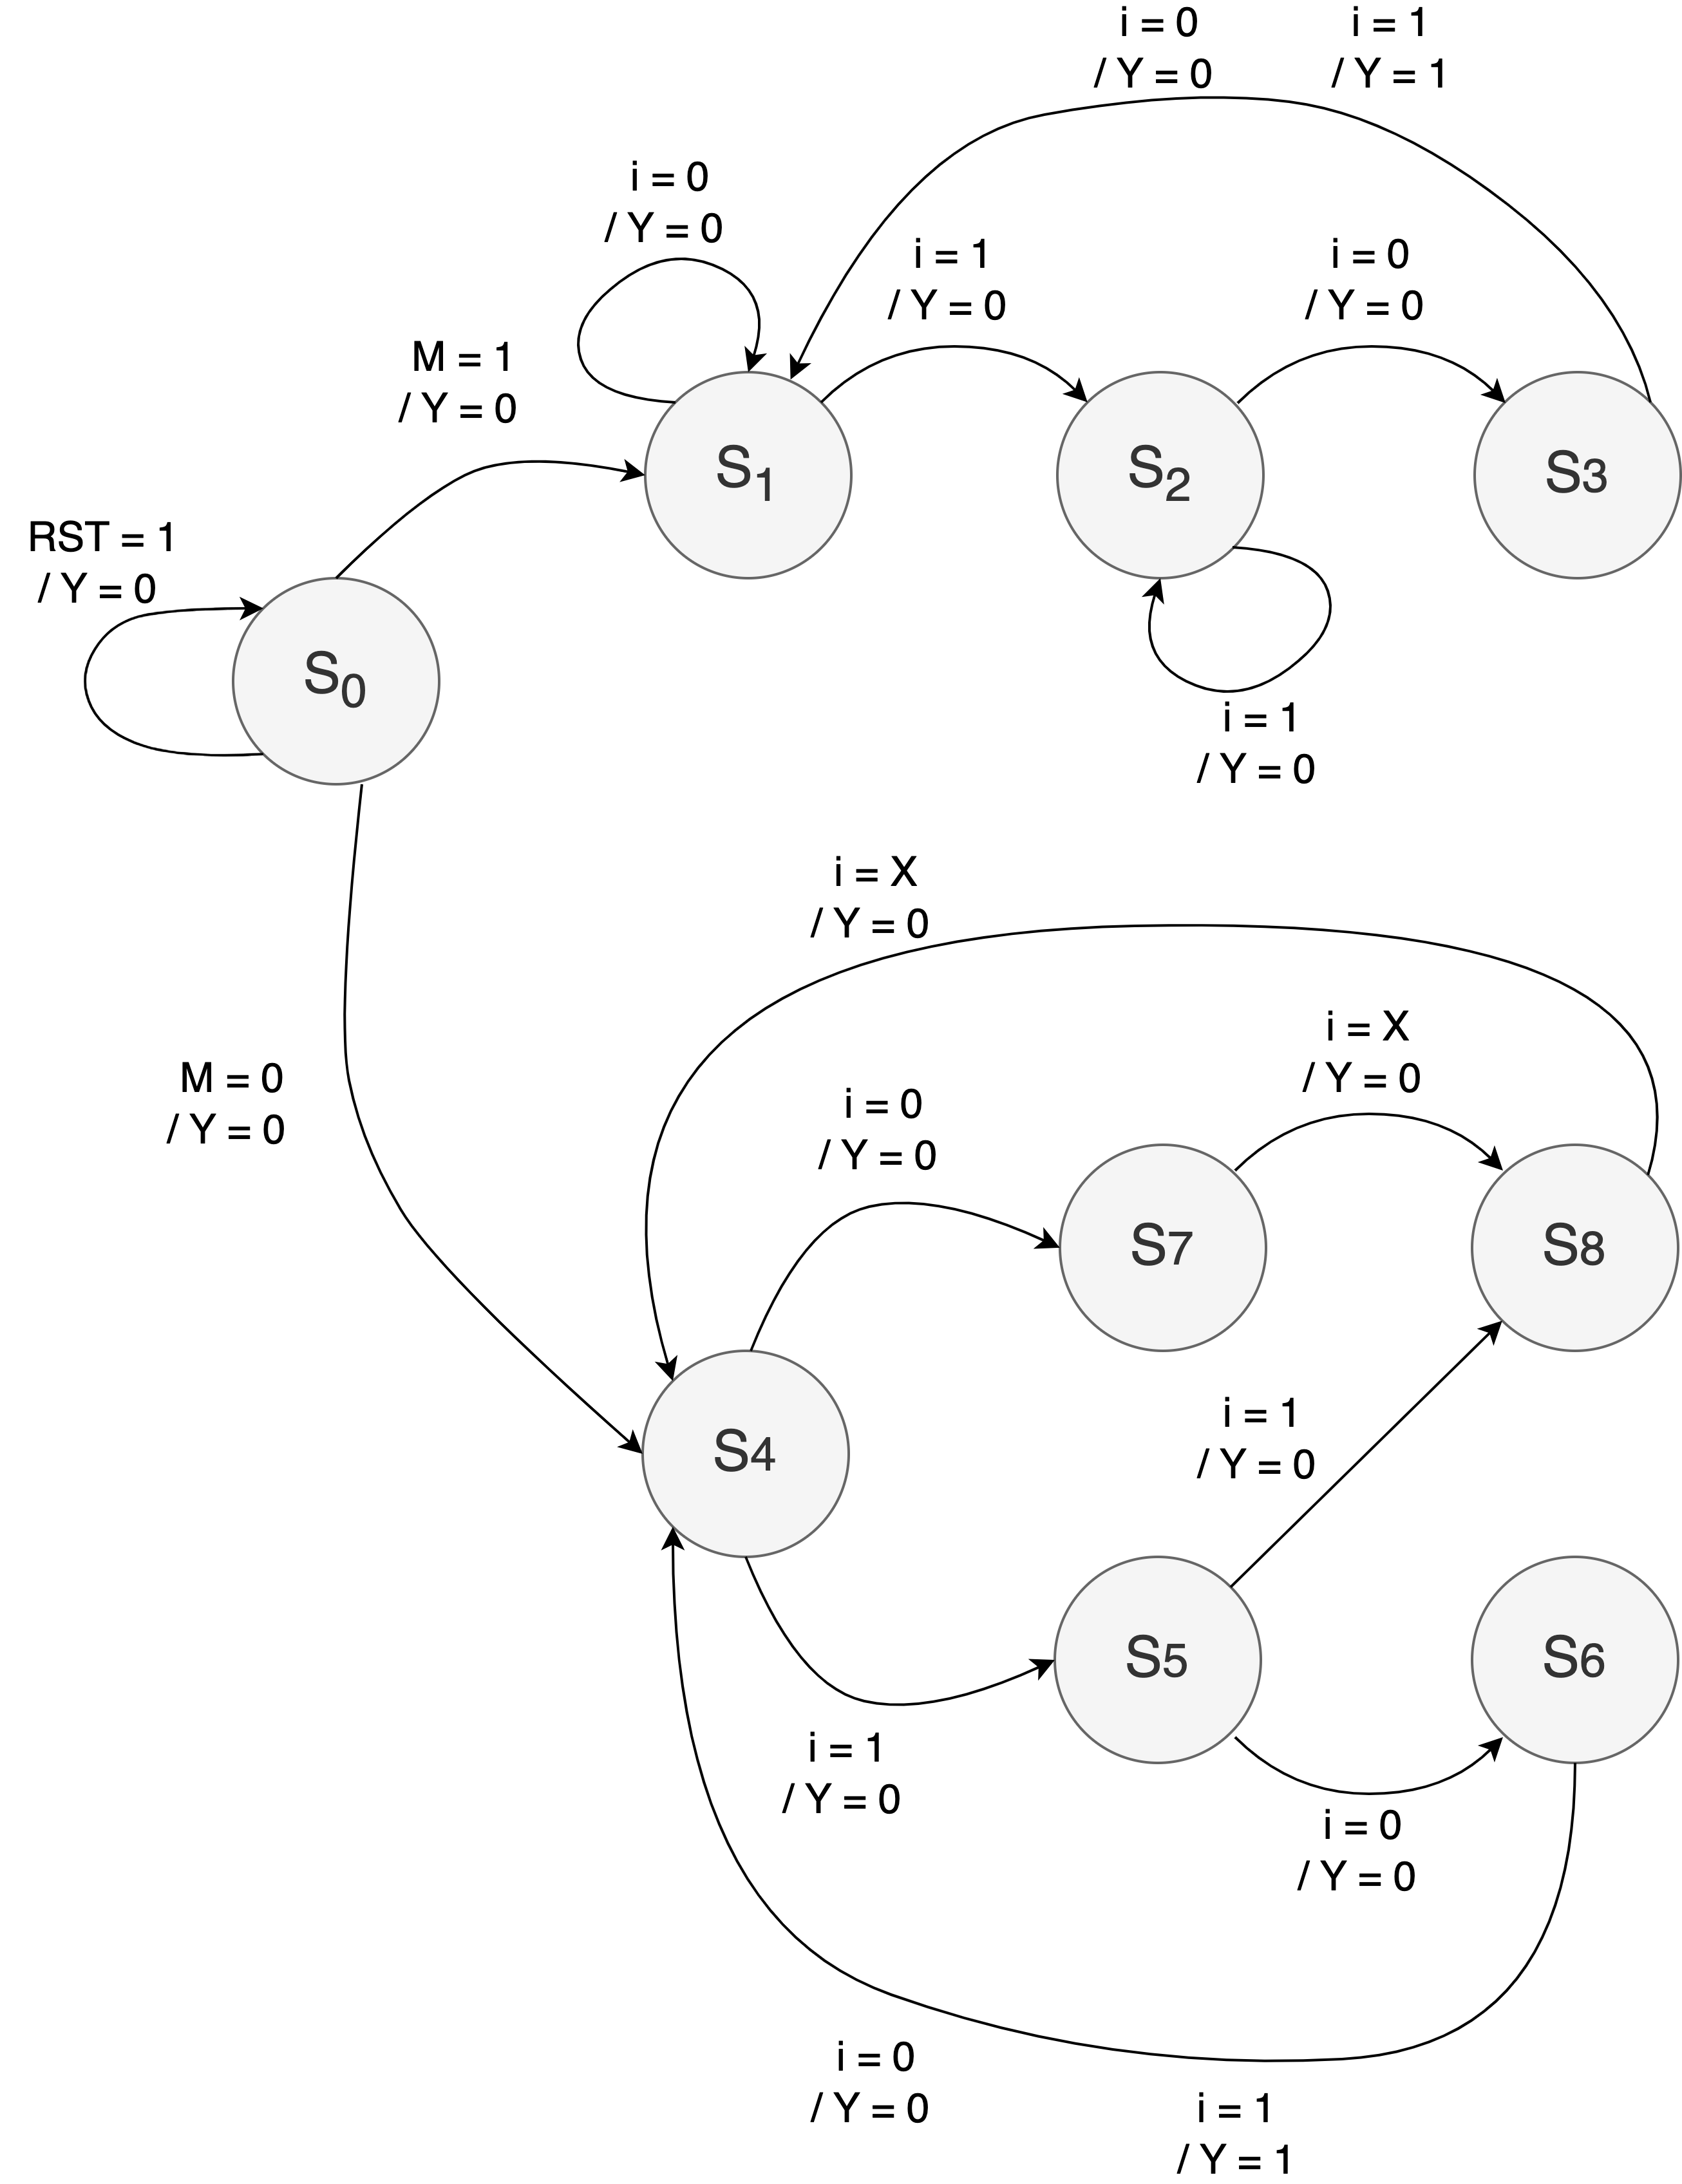
\includegraphics[width=0.7\textwidth]{img/automa_riconoscitore}
	\caption{Automa riconoscitore di sequenza}
	\label{aut_ric_seq} 
\end{figure}

\subsection{Implementazione}
Per l'implementazione VHDL dell'automa, si dichiarano dapprima gli ingressi
\begin{itemize}
    \item \texttt{RST}: permette il reset della macchina, portandola allo stato $S_0$;
    \item \texttt{A}: rappresenta l'abilitazione, ovvero il clock;
    \item \texttt{i}: è l'ingresso;
    \item \texttt{M}: permette di selezionare con quale modalità far lavorare la macchina: se $M=0$ effettua il riconoscimento a gruppi di tre bit per volta; se $M=1$ effettua il riconoscimento un bit alla volta
\end{itemize}
L'uscita è rappresentata dal segnale \texttt{Y}.\\
L'architettura è costruita con un approccio comportamentale e vi è una variazione di stato ad ogni fronte di salita del clock (\texttt{A}).\\
Si vuole notare che il segnale \texttt{RST} è sincrono.

\begin{code}
    \inputminted[frame=lines, framesep=2mm, baselinestretch=1.2, bgcolor=LightGray, fontsize=\footnotesize, linenos]{vhdl}{vhdl_files/riconoscitore.vhdl}
    \caption{riconoscitore.vhdl}
    \label{lst:RIC}
\end{code}

\subsection{Simulazione}
Per effettuare la simulazione, è stato necessario il seguente testbench.
\begin{code}
    \inputminted[frame=lines, framesep=2mm, baselinestretch=1.2, bgcolor=LightGray, fontsize=\footnotesize, linenos]{vhdl}{vhdl_files/riconoscitore_tb.vhdl}
    \caption{riconoscitore\_tb.vhdl}
    \label{lst:RIC}
\end{code}

Gli ingressi sono i seguenti:
\begin{itemize}
    \item $M=1$:
        \begin{itemize}
            \item 1, 1, 0, 1, 0, 0, 1, 0, 1
        \end{itemize}
    \item $M=0$:
        \begin{itemize}
            \item 1, 1, 0, 1, 0, 1, 1, 0, 1
        \end{itemize}
\end{itemize}

Il risultato è il seguente:

\begin{figure}[H]
	\centering
	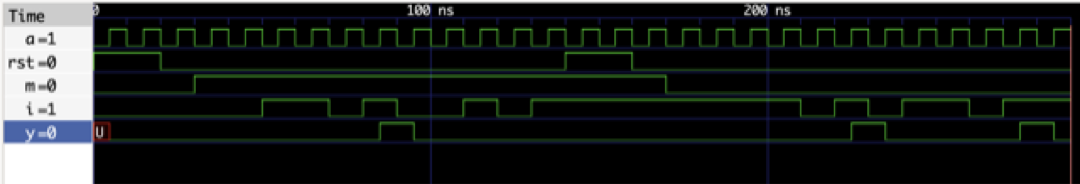
\includegraphics[width=1\textwidth]{img/Sim_RIC}
	\caption{Simulazione Riconosciore}
	\label{aut_ric_seq} 
\end{figure}

%\begin{itemize}
%    \item \textbf{Stato S0}:
%        \begin{itemize}
%            \item se $i=0$, si rimane in \textbf{S0};
%            \item se $i=1$, si raggiunge lo stato \textbf{S1};
%        \end{itemize}
%    \item \textbf{Stato S1}:
%        \begin{itemize}
%            \item se $i=0$, si raggiunge lo stato \textbf{S2};
%            \item se $i=1$ e $M=0$ si rimane nello stato \textbf{S1}
%        \end{itemize}
%    \item \textbf{Stato S2}:
%        \begin{itemize}
%            \item se $i=0$ e $M=1$, si raggiunge lo stato \textbf{S0}
%            \item se $i=1$ si raggiunge lo stato \textbf{S3}
%        \end{itemize}
%    \item \textbf{Stato S3}:
%        \begin{itemize}
%            \item se $M=1$, si raggiunge lo stato \textbf{S0} con uscita $Y=1$
%            \item se $M=0$, si raggiunge lo stato \textbf{S1} con uscita $Y=1$
%        \end{itemize}
%\end{itemize}

\section{Implementazione su board del punto precedente}
\subsection{Traccia}
 Sintetizzare e implementare su board la rete sviluppata al punto precedente, utilizzando uno switch S1 per codificare l’input i e uno switch S2 per codificare il modo M, in combinazione con due bottoni B1 e B2 utilizzati rispettivamente per acquisire l’input da S1 e S2 in sincronismo con il segnale di tempificazione A, che 
deve essere ottenuto a partire dal clock della board. Infine, l’uscita Y può essere codificata utilizzando un led.
\subsection{Implementazione}
Il Riconoscitore di sequenza viene ripreso dal punto precedente, di conseguenza il suo codice viene importato nel progetto senza variazioni.\\
Per gestire il funzionamento di tale sistema su board, prima di tutto si rende necessario l'utilizzo di un divisore di frequenze che ha la funzione di generare un segnale di clock con una frequenza più bassa rispetto al clock di ingresso. In particolare il  processo implementato genera un clock di uscita con una frequenza pari a quella di ingresso divisa per il valore di \textit{DIVISOR}.
Si mostra il codice:
\begin{code}
    \inputminted[frame=lines, framesep=2mm, baselinestretch=1.2, bgcolor=LightGray, fontsize=\footnotesize, linenos]{vhdl}{vhdl_files/seq_rec_Board/freq_div.vhd}
    \caption{frequency\_divider.vhdl}
    \label{lst:SR_beh}
\end{code}
Per la gestione degli input tramite i bottoni della board, è stata realizata una unità di controllo; si usa lo $switch[0]$ unito al bottone \textit{BTNL} per l'ingresso "i", e lo $switch[1]$ unito al bottone \textit{BTNR} per l'ingresso "M". Si è scelto inoltre di mostrare le variazioni del clock sul $led[0]$, in modo da poter inserire correttamente gli input in corrispondenza del fronte di salita. L'uscita viene invece visualizzata sul $led[1]$.
\begin{code}
    \inputminted[frame=lines, framesep=2mm, baselinestretch=1.2, bgcolor=LightGray, fontsize=\footnotesize, linenos]{vhdl}{vhdl_files/seq_rec_Board/control_unit.vhd}
    \caption{control\_unit.vhdl}
    \label{lst:SR_beh}
\end{code}
Il codice del sistema su board, nel suo complesso, è stato realizzato seguendo un approccio di tipo strutturale:
\begin{code}
    \inputminted[frame=lines, framesep=2mm, baselinestretch=1.2, bgcolor=LightGray, fontsize=\footnotesize, linenos]{vhdl}{vhdl_files/seq_rec_Board/RecOnBoard.vhd}
    \caption{Riconoscitore su board in vhdl}
    \label{lst:SR_beh}
\end{code}


\chapter{Esercizio 4}
\section{Shift Register - Approccio comportamentale}
Si vuole implementare uno Shift Register con approccio comportamentale, la cui dimensione è $N$.\\
Tale macchina ha come ingresso un valore $y$ con il quale si può scegliere di fare shift verso destra o sinistra e di fare shift di uno o due bit.
\subsection{Progetto e architettura}
La macchina da implementare è la seguente:
\begin{figure}[H]
	\centering
	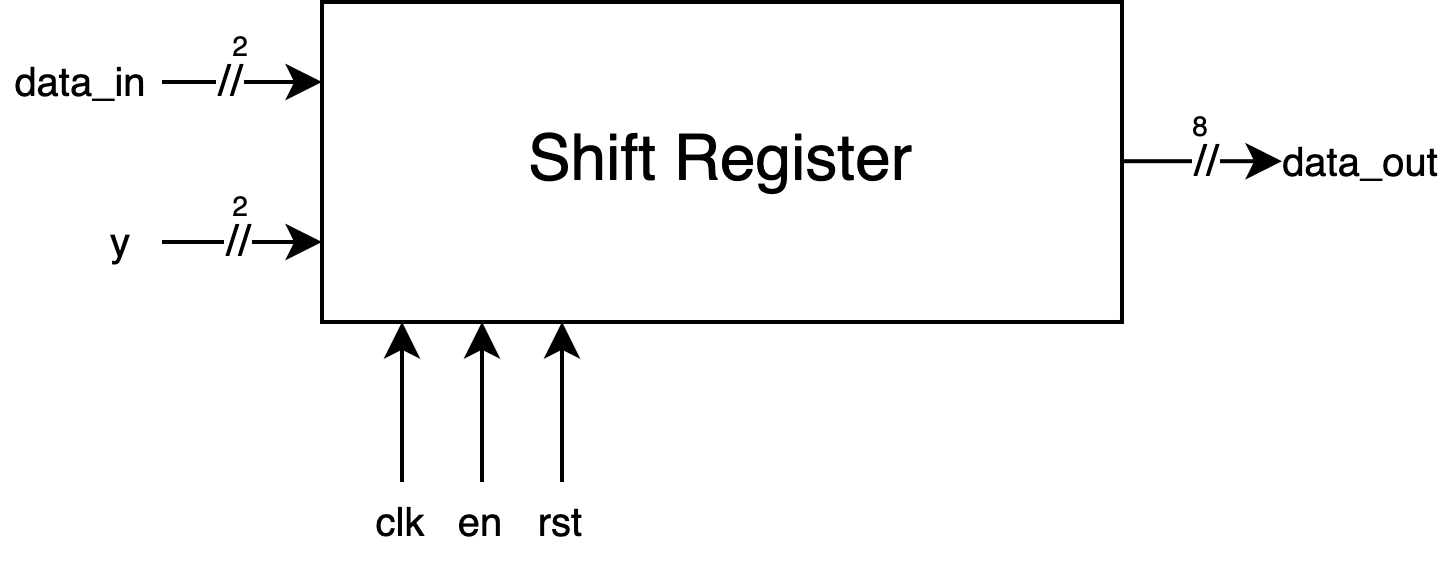
\includegraphics[width=0.7\textwidth]{img/shift_register}
	\caption{Shift Register}
	\label{shf_reg} 
\end{figure}
Dall'immagine si può notare che è stato scelto $N=8$.\\
Gli ingressi sono i seguenti:
\begin{itemize}
    \item \texttt{clk}: il clock, necessario per la tempificazione. La macchina lavorerà sul fronte di salita;
    \item \texttt{en}: l'abilitazione, la quale permette di abilitare o disabilitare la macchina;
    \item \texttt{rst}: reset sincrono della macchina;
    \item \texttt{y}: vettore di 2 elementi che sceglie la modalità di funzionamento della macchina; in particolare:
        \begin{itemize}
            \item $y=00$: shift a sinistra di 1;
            \item $y=01$: shift a sinistra di 2;
            \item $y=10$: shift a destra di 1;
            \item $y=11$: shift a destra di 2;
        \end{itemize}
    \item  \texttt{data\_in}: rappresenta i dati in ingresso; esso è un vettore di due elementi poiché quando vi è la necessità di fare uno shift di 2, si ha bisogno di due bit
\end{itemize}
L'uscita della macchina è \texttt{data\_out}, vettore di 8 bit.
\subsection{Implementazione}
L'implementazione è la seguente
\begin{code}
    \inputminted[frame=lines, framesep=2mm, baselinestretch=1.2, bgcolor=LightGray, fontsize=\footnotesize, linenos]{vhdl}{vhdl_files/shift_registrer_beh.vhdl}
    \caption{shift\_register\_beh.vhdl}
    \label{lst:SR_beh}
\end{code}

\subsection{Simulazione}
Per effettuare la simulazione, si utilizza il seguente testbench:
\begin{code}
    \inputminted[frame=lines, framesep=2mm, baselinestretch=1.2, bgcolor=LightGray, fontsize=\footnotesize, linenos]{vhdl}{vhdl_files/shift_register_beh_tb.vhdl}
    \caption{shift\_register\_beh\_tb.vhdl}
    \label{lst:SR_beh_tb}
\end{code}
\noindent Il risultato della simulazione è il seguente:

\begin{figure}[H]
	\centering
	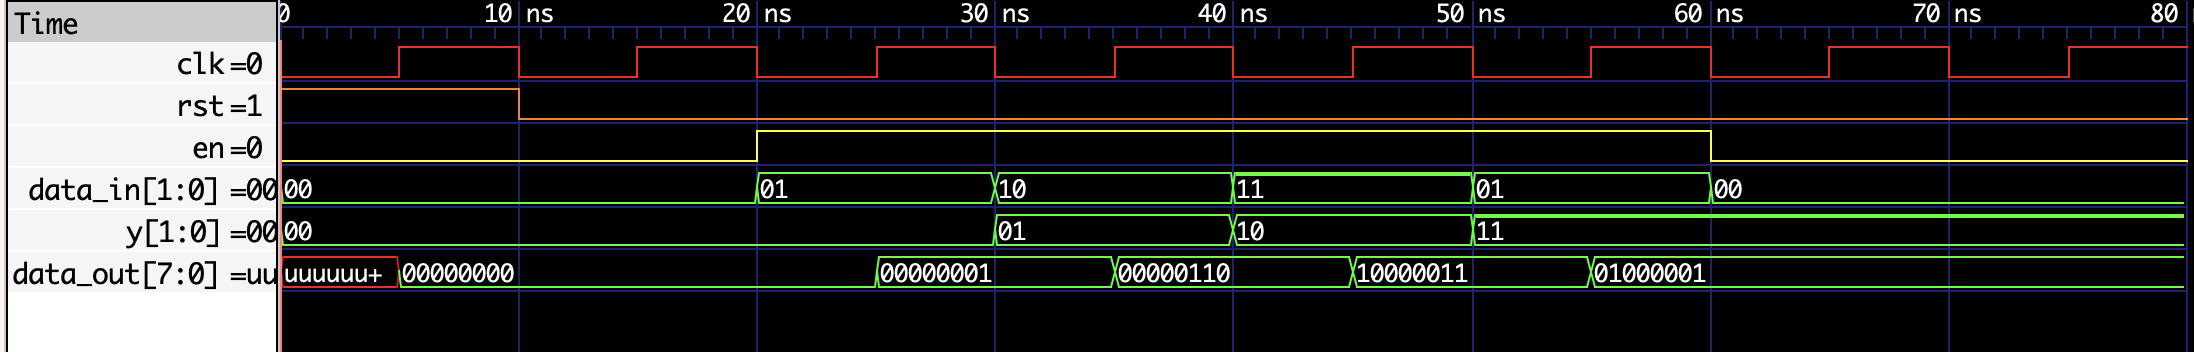
\includegraphics[width=1\textwidth]{img/simulazione_shift_register.png}
	\caption{Simulazione Shift Register con approccio comportamentale}
	\label{shf_reg_beh_sim} 
\end{figure}
Si può facilmente notare dall'immagine che la macchina lavora come desiderato: ad ogni fronte di salita del clock e quando l'abilitazione è alta, in base alla modalità di lavoro, shifta a destra o a sinistra, di uno o due bit.

\section{Shift Register - Approccio strutturale}
Si vuole riprogettare la macchina precedente, figura \ref{shf_reg}, utilizzando un approccio strutturale.\\
Le componenti della macchina sono 8 registri da 1 bit e 8 mux 4:1.\\
Si sono scelti 8 registri poiché in tale esempio si realizza un registro da 8 bit ($N=8$).
\subsection{Progetto e architettura}
\subsubsection{Registro da un bit}
Il primo componente necessario è il registro da un bit.
\begin{figure}[H]
	\centering
	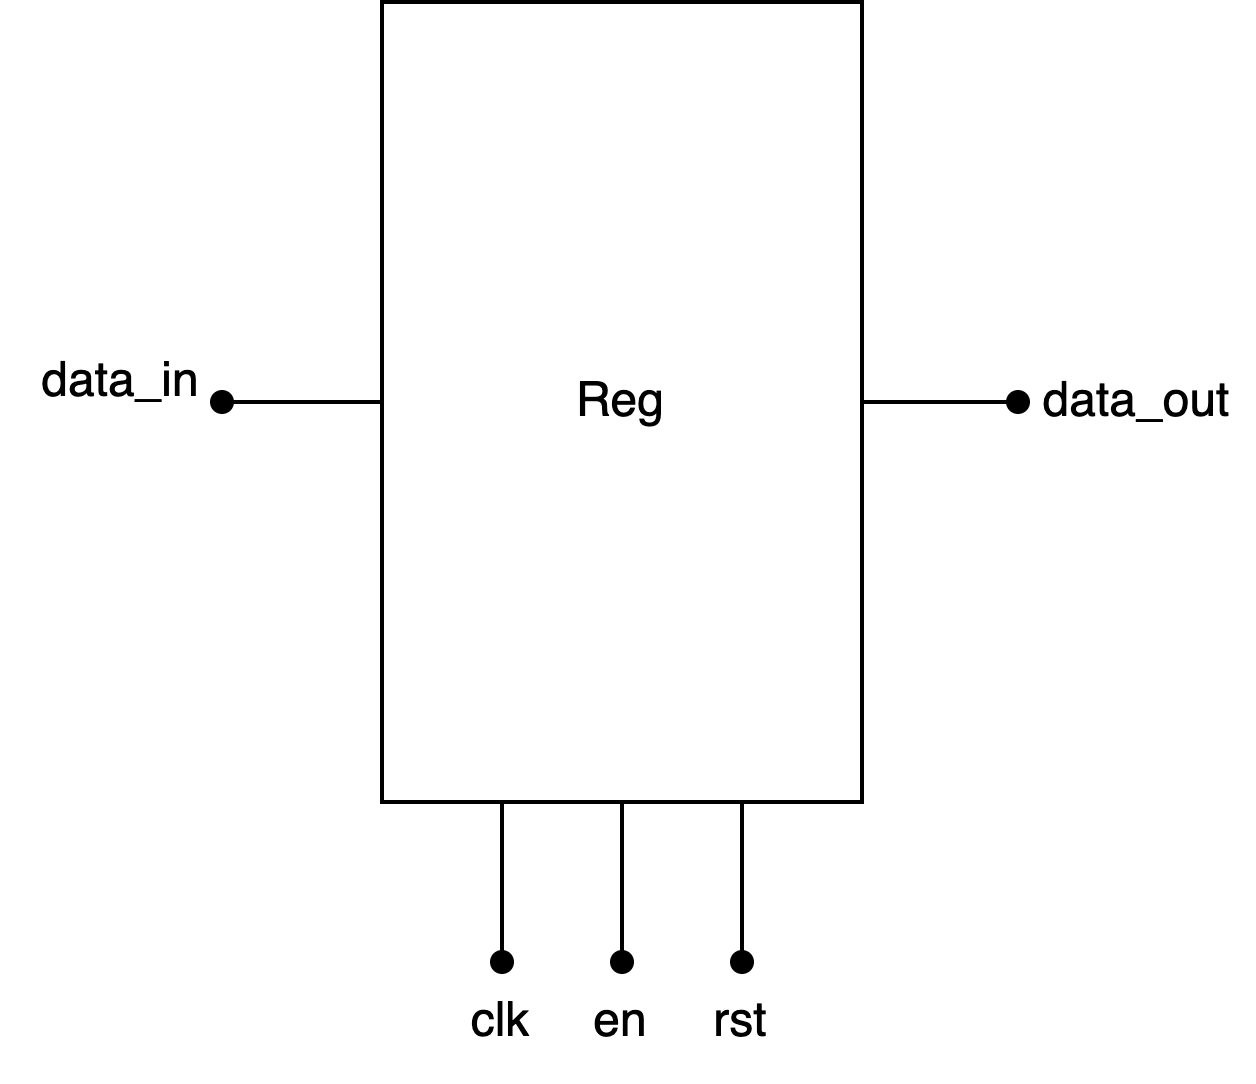
\includegraphics[width=0.7\textwidth]{img/reg.png}
	\caption{Registro da 1 bit}
	\label{shf_reg_beh_sim} 
\end{figure}
Gli ingressi di tale componente sono i seguenti:
\begin{itemize}
    \item \texttt{data\_in}: bit in ingresso, che verrà memorizzato nel registro;
    \item \texttt{clk}: il clock per la tempificazione; il registro lavora sul fronte di salita di quest'ultimo;
    \item \texttt{en}: segnale di abilitazione; il registro memorizza il bit in ingresso solo quando tale segnale è alto;
    \item \texttt{rst}: segnale che quando è alto resetta il registro, portando il valore al suo interno a 0; il reset è sincrono.
\end{itemize}
La sua uscita è \texttt{data\_out}, che altro non rappresenta il bit memorizzato nel registro.
\subsubsection{Mux 4:1}
Il secondo componente è il mux 4:1.\\
Tramite quest'ultimo si decide qual è l'ingresso di un registro, attraverso la selezione.\\
\begin{figure}[H]
	\centering
	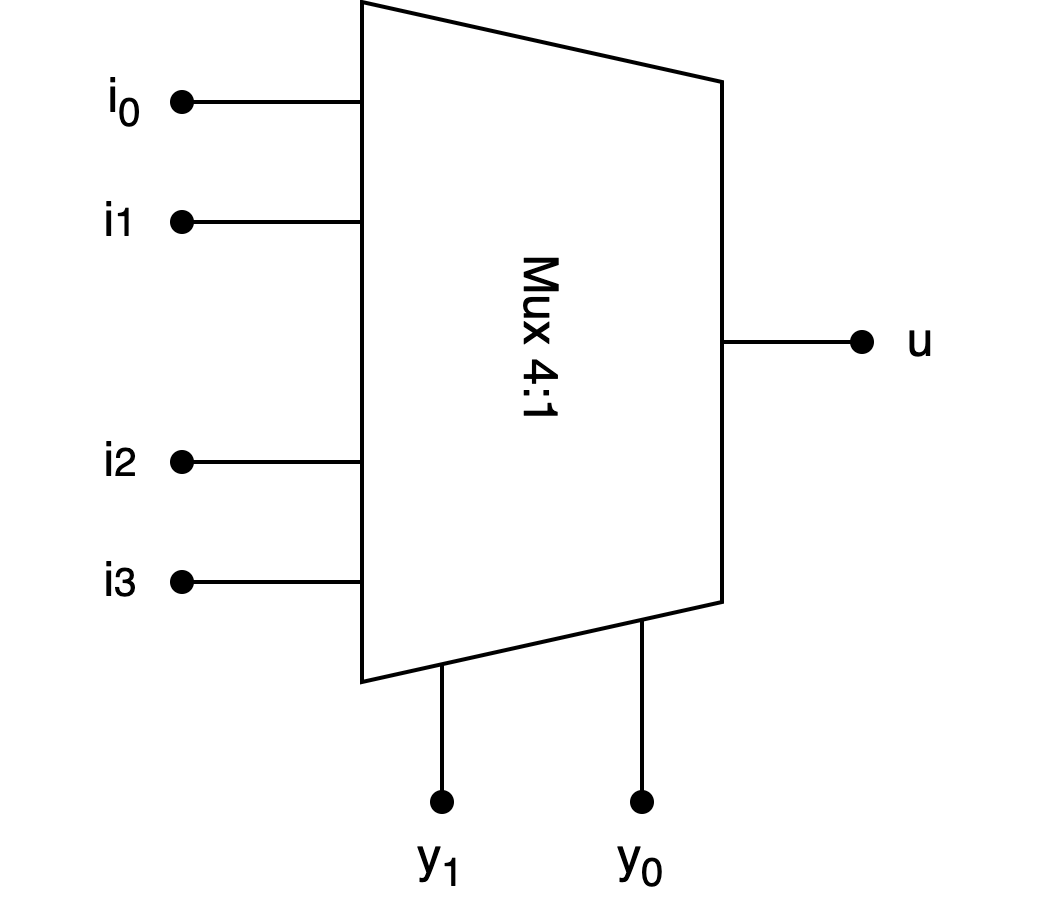
\includegraphics[width=0.5\textwidth]{/mux_41_sr.png}
	\caption{Mux 4:1}
	\label{mux_41_sr} 
\end{figure}
\noindent Tale multiplexer lavora seguendo la seguente tabella:
\begin{table}[h!]
    \centering
    \begin{tabular}{||c|c||c||}
        \hline
        \hline
        $\mathbf{y_1}$ & $\mathbf{y_0}$ & $\mathbf{u}$ \\
        \hline
        0 & 0 & $\mathbf{i_0}$ \\
        \hline
        0 & 1 & $\mathbf{i_1}$ \\
        \hline
        1 & 0 & $\mathbf{i_2}$ \\
        \hline
        1 & 1 & $\mathbf{i_3}$ \\
        \hline
        \hline 
    \end{tabular}
    \caption{Tabella di verità del multiplexer 4:1 per lo Shift Register}
    \label{tab:mux_4:1_sr}
\end{table}
Si può banalmente notare che l'uscita altro non è che uno dei 4 ingressi del multiplexer, scelto tramite la selezione.

Si può ora comporre lo Shift Register.\\
Facendo gli opportuni collegamenti, si ottiene il seguente schema
\begin{figure}[H]
	\centering
	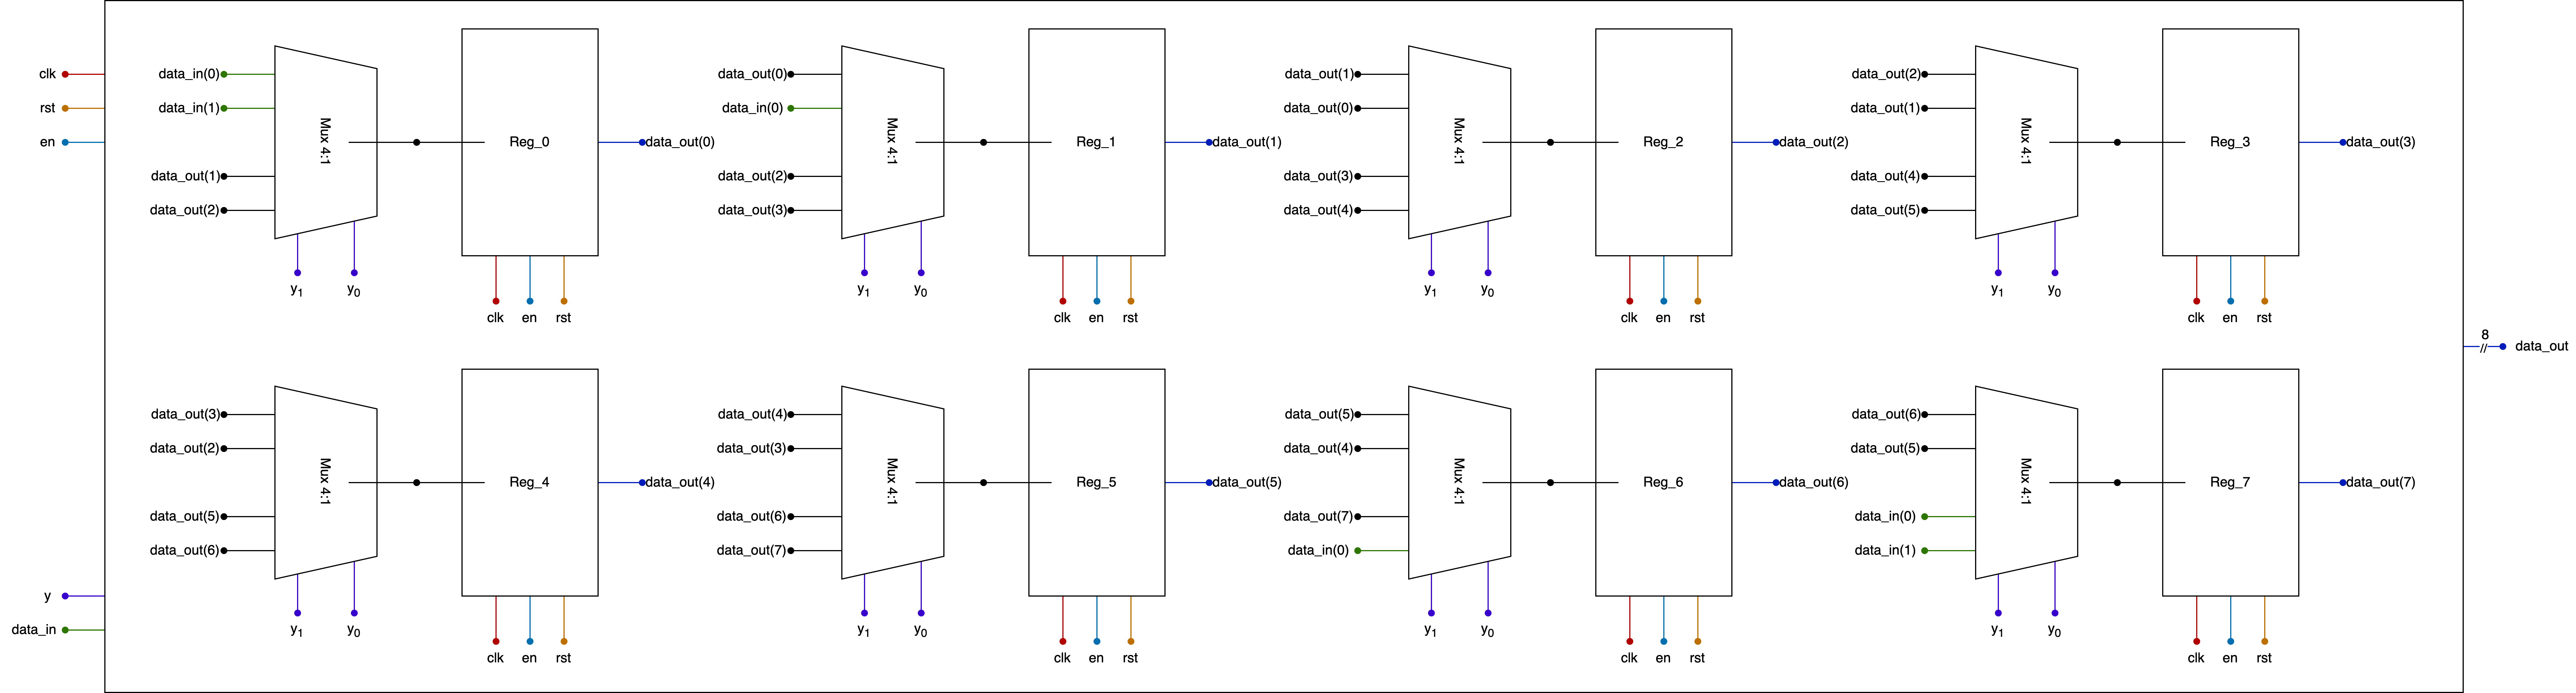
\includegraphics[width=1\textwidth]{shiftregister_str.png}
	\caption{Shift Register con approccio strutturale}
	\label{mux_41_sr} 
\end{figure}
Gli ingressi e l'uscita dello Shift Register sono identici a quelli visti nell'esercizio precedente.\\
Quello che si vuole mettere in evidenzia in questo caso è come tali ingressi siano collegati con le strutture interni: in particolare si vede che \texttt{y}, che sceglie la modalità di lavoro della macchina, è collegato alla selezione dei multiplexer, mentre \texttt{data\_in}, è collegato solo ai primi due e agli ultimi due multiplexer.\\
I restanti sono collegati direttamente ai registri.

\subsection{Implementazione}
Si vuole ora procedere con l'implementazione in VHDL.\\
Partendo dal registro, si ha:
\begin{code}
    \inputminted[frame=lines, framesep=2mm, baselinestretch=1.2, bgcolor=LightGray, fontsize=\footnotesize, linenos]{vhdl}{vhdl_files/Cap_4/register.vhdl}
    \caption{register.vhdl}
    \label{lst:rgt_one_bit}
\end{code}
\noindent Si prosegue con il multiplexer 4:1
\begin{code}
    \inputminted[frame=lines, framesep=2mm, baselinestretch=1.2, bgcolor=LightGray, fontsize=\footnotesize, linenos]{vhdl}{vhdl_files/Cap_4/mux_4_1.vhdl}
    \caption{mux\_4\_1.vhdl}
    \label{lst:mux_4_1_sr}
\end{code}
\noindent Implementate le componenti base per il progetto, si prosegue con lo Shift Register:
\begin{code}
    \inputminted[frame=lines, framesep=2mm, baselinestretch=1.2, bgcolor=LightGray, fontsize=\footnotesize, linenos]{vhdl}{vhdl_files/Cap_4/shift_register.vhdl}
    \caption{shift\_register.vhdl}
    \label{lst:sr_s}
\end{code}
Si può notare come nella architettura, sono state prima generate le componenti e solo dopo sono stati effettuati i vari collegamenti, utilizzando variabili ausiliarie.

\subsection{Simulazione}
Per effettuare la simulazione, si implementa il seguente testbench
\begin{code}
    \inputminted[frame=lines, framesep=2mm, baselinestretch=1.2, bgcolor=LightGray, fontsize=\footnotesize, linenos]{vhdl}{vhdl_files/Cap_4/tb_shift_register.vhdl}
    \caption{tb\_shift\_register.vhdl}
    \label{lst:tb_sr}
\end{code}
Lanciando la simulazione, il risultato è il seguente:
\begin{figure}[H]
	\centering
	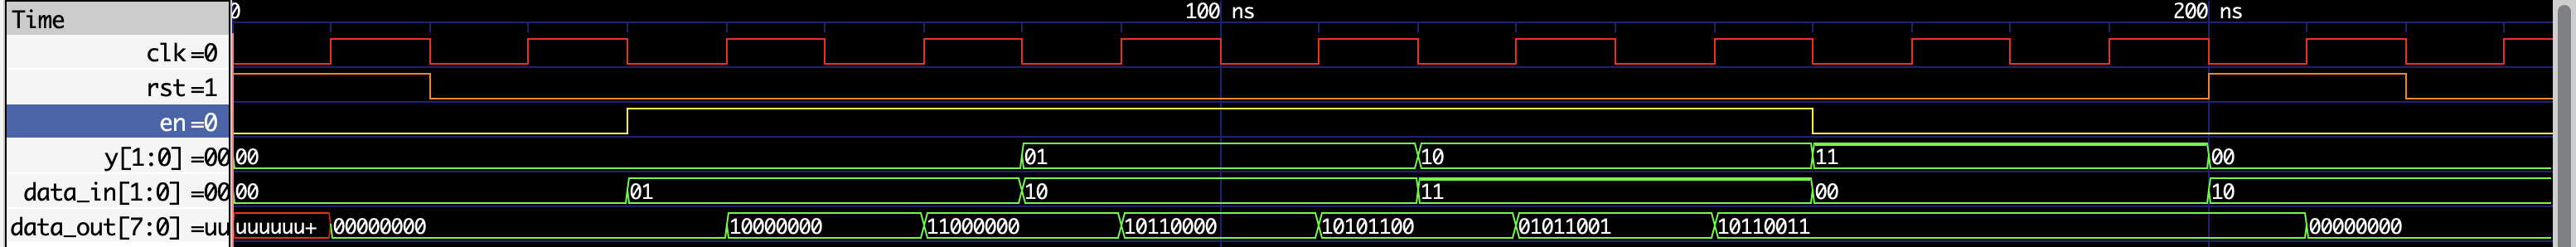
\includegraphics[width=1\textwidth]{img/sim_shift_register_str.png}
	\caption{Simulazione dello Shift Register con approccio strutturale}
	\label{sim_sr_str} 
\end{figure}
Si nota chiaramente un corretto funzionamento della macchina.

\chapter{Esercizio 5}
\section{Cronometro}
Si vuole progettare, implementare e testare un cronometro, in grado di scandire secondi, minuti e ore, a partire da una base dei tempi prefissata (clock). \\
Si vuole inoltre che l'inizializzazione del cronometro possa essere fatta anche con un valore iniziale, espresso in ore, minuti e secondi, mediante un ingresso di \texttt{set}, e deve prevedere un ingresso di \texttt{reset} per azzerare il tempo.

\subsection{Progettazione}
Per la progettazione di tale macchina, si utilizza un approccio strutturale.\\
In linea generale, si parte da un flip-flop D per la composizione di contatori di modulo 64 e modulo 32. Questi ultimi saranno necessari per la progettazione di due contatori modulo 60 e un contatore modulo 24, rispettivamente.\\
Questi ultimi tre, collegati opportunamente, andranno a comporre il cronometro.

\subsubsection{Flip-Flop D}
Il Flip-Flop D è progettato come segue:
\begin{figure}[H]
	\centering
	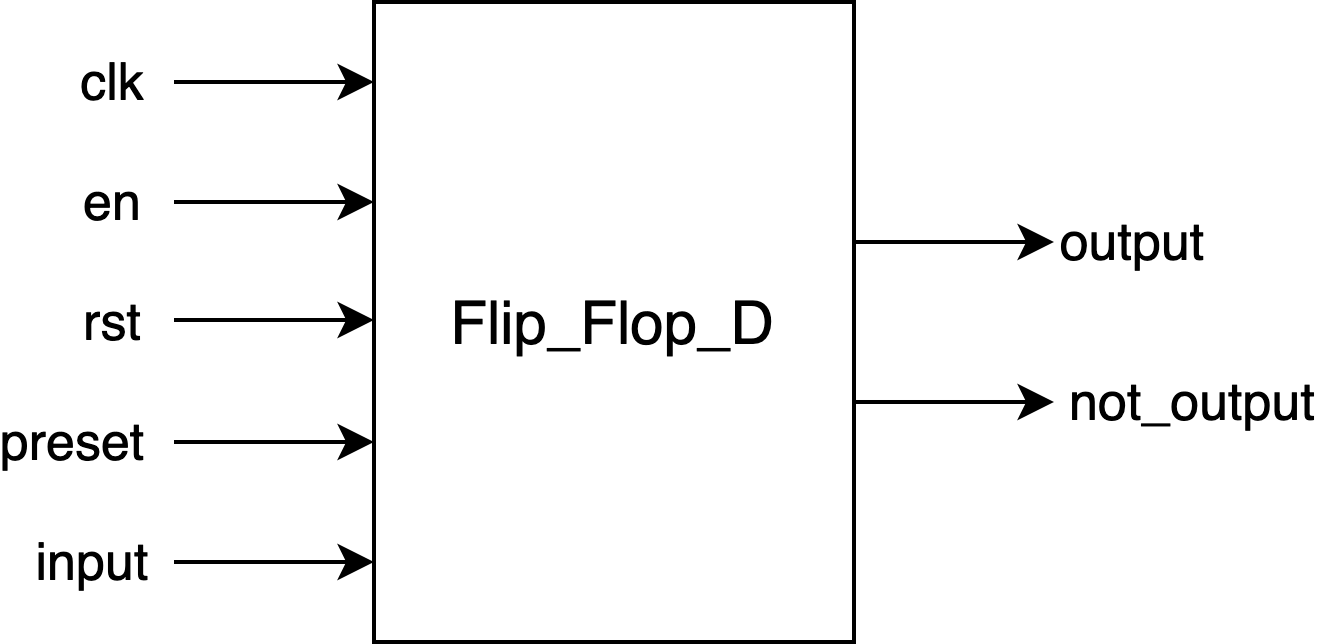
\includegraphics[width=0.7\textwidth]{img/ffD}
	\caption{Flip-Flop D}
	\label{ffd} 
\end{figure}
La macchina lavora sul fronte di salita del clock e quando il valore \texttt{en} è alto. \\
Ha due uscite, la prima \texttt{output} presenta in uscita ciò che è memorizzato nel Flip-Flop, mentre \texttt{not\_output}, presenta il negato.

\subsubsection{Contatore modulo 64}
Il contatore modulo 64 che si vuole progettare è il seguente:
\begin{figure}[H]
	\centering
	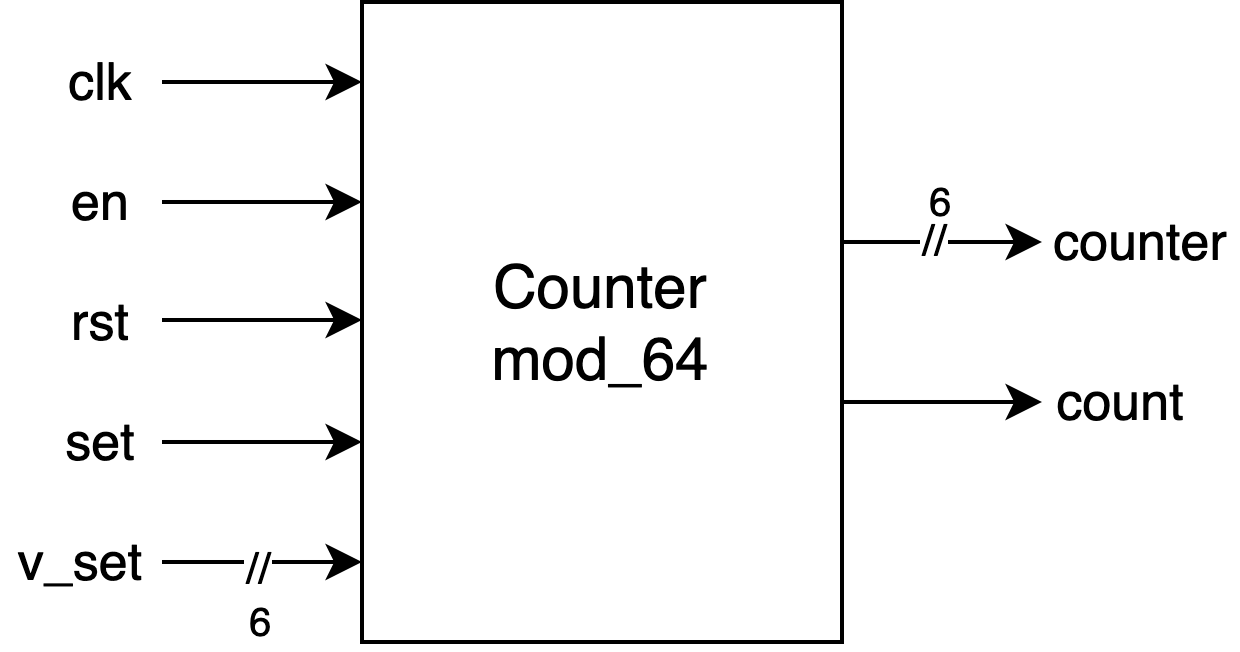
\includegraphics[width=0.7\textwidth]{img/counter_64}
	\caption{Contatore modulo 64}
	\label{cnt_64} 
\end{figure}
Gli ingessi sono:
\begin{itemize}
    \item \texttt{clk}: clock per la tempificazione;
    \item \texttt{en}: segnale di abilitazione;
    \item \texttt{rst}: segnale di reset;
    \item \texttt{set} e \texttt{v\_set}: segnali necessari per il setting del valore di partenza
\end{itemize}
Le uscite sono \texttt{counter}, che altro non è il conteggio, e \texttt{count}, uscita necessaria per permettere il collegamento con altri contatori.\\

\noindent Si vuole progettare tale macchina strutturalmente, utilizzando come componente base il Flip-Flop D.\\
Per far ciò si collegano parallelamente cinque Flip-Flop D, nel modo seguente:
\clearpage
\begin{sidewaysfigure}[ht]
	\centering
	
\includegraphics[width=1\textwidth]{img/counter_mod_64_str.png}
	\caption{Contatore modul0 64 - approccio strutturale}
	\label{cnt_64_str} 
\end{sidewaysfigure}
\clearpage

\subsubsection{Contatore modulo 32}
Il contatore modulo 32 è esteriormente identico a quello modulo 64:
\begin{figure}[H]
	\centering
	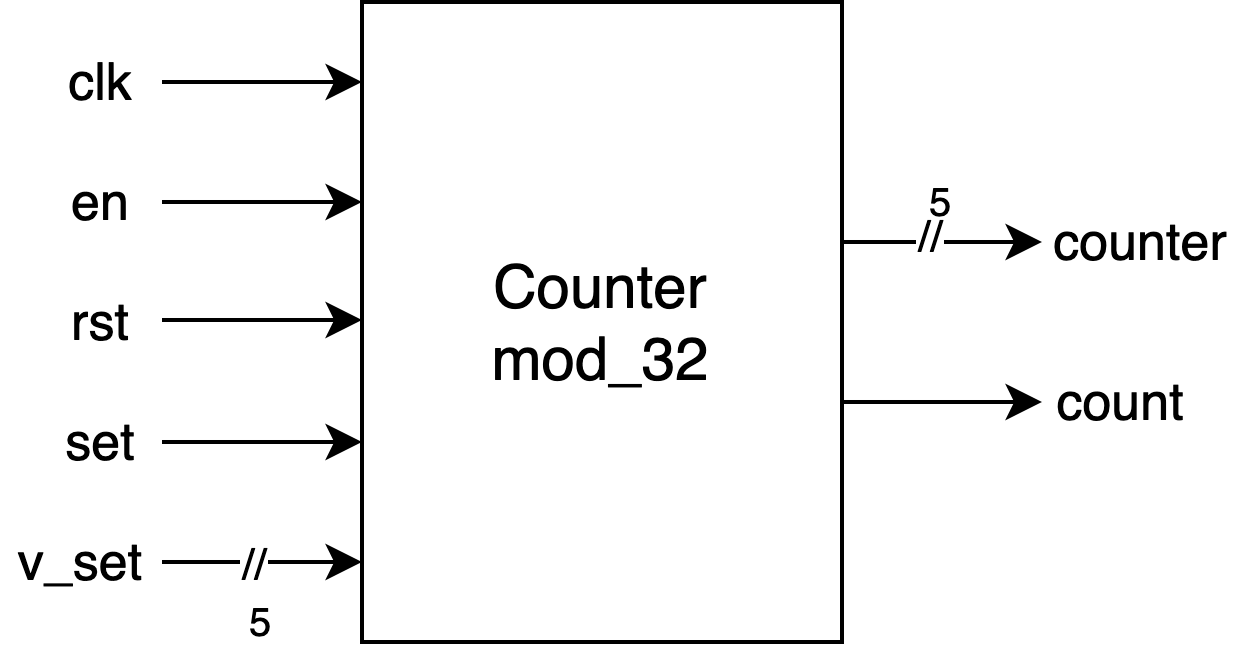
\includegraphics[width=0.7\textwidth]{img/counter_mod_32.png}
	\caption{Contatore modulo 32}
	\label{cnt_32} 
\end{figure}

\noindent Analogamente al caso precedente, si compone strutturalmente con i Flip-Flop D:
\clearpage
\begin{sidewaysfigure}[ht]
	\centering
	
\includegraphics[width=1\textwidth]{img/counter_mod_32_str.png}
	\caption{Contatore modulo 32 - approccio strutturale}
	\label{cnt_32_str} 
\end{sidewaysfigure}
\clearpage

\subsubsection{Contatore modulo 60}
Per progettare un contatore modulo 60, si parte da un contatore modulo 64 facendo in modo che ogni qual volta raggiunga 59 si resetti.
\begin{figure}[H]
	\centering
	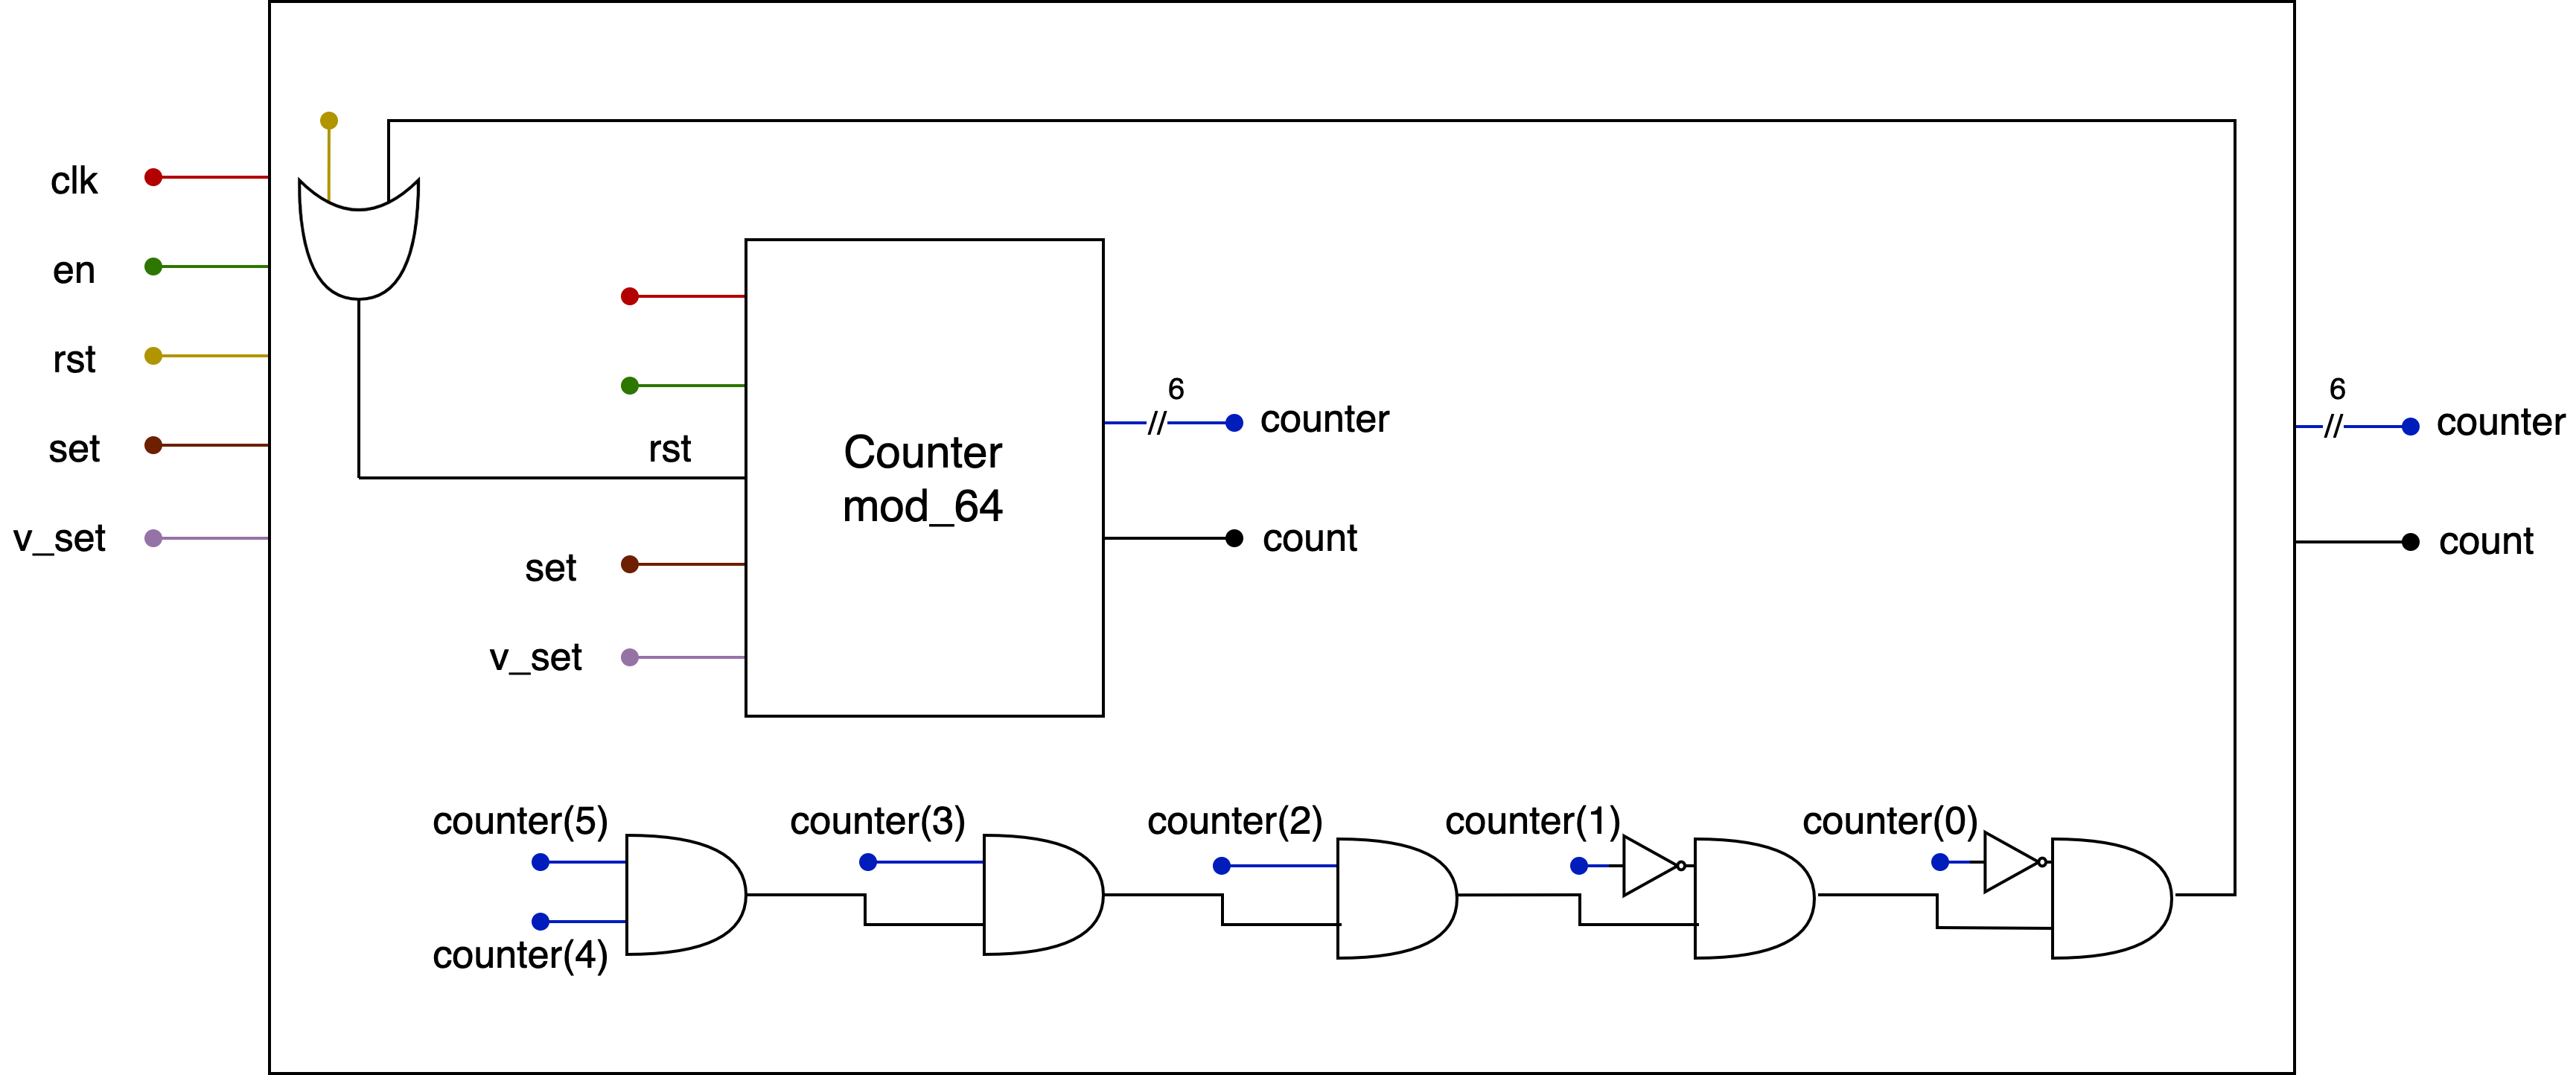
\includegraphics[width=1\textwidth]{img/counter_mod_60.png}
	\caption{Contatore modulo 60}
	\label{cnt_60} 
\end{figure}

\subsubsection{Contatore modulo 24}
Analogamente al contatore precedente, si realizza il contatore modulo 24 utilizzando il contatore modulo 32 in modo che si resetti ogni qualvolta raggiunga 23
\begin{figure}[H]
	\centering
	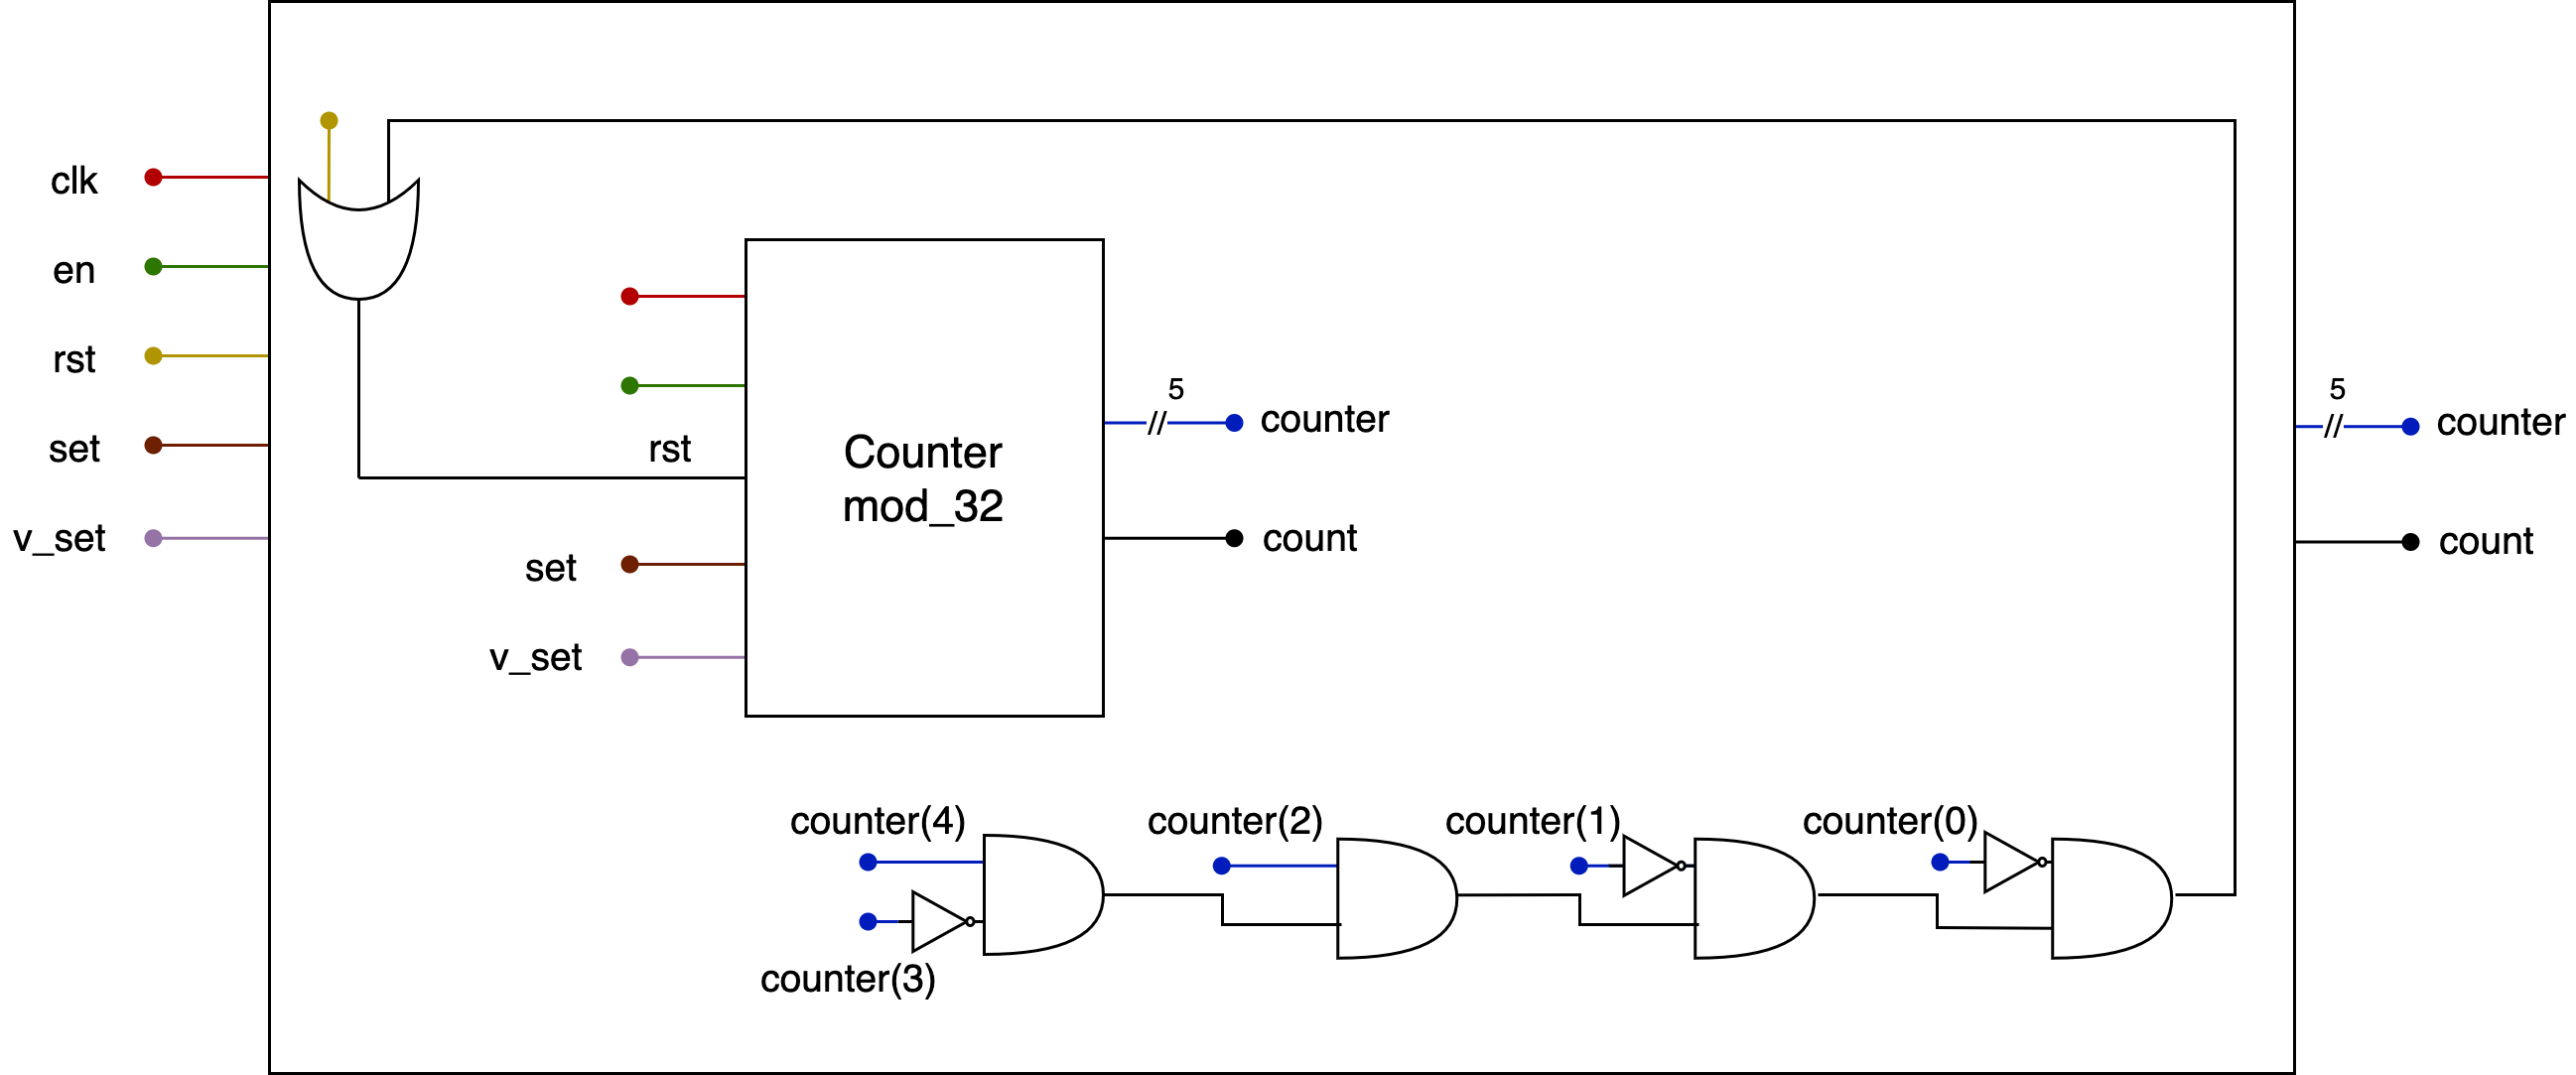
\includegraphics[width=1\textwidth]{img/counter_mod_24.png}
	\caption{Contatore modulo 24}
	\label{cnt_60} 
\end{figure}

\subsubsection{Cronometro}
Si possono ora effettuare i collegamenti per creare un cronometro: ovviamente servono due contatori modulo 60 per secondi e minuti, e un contatore modulo 24:
\begin{figure}[H]
	\centering
	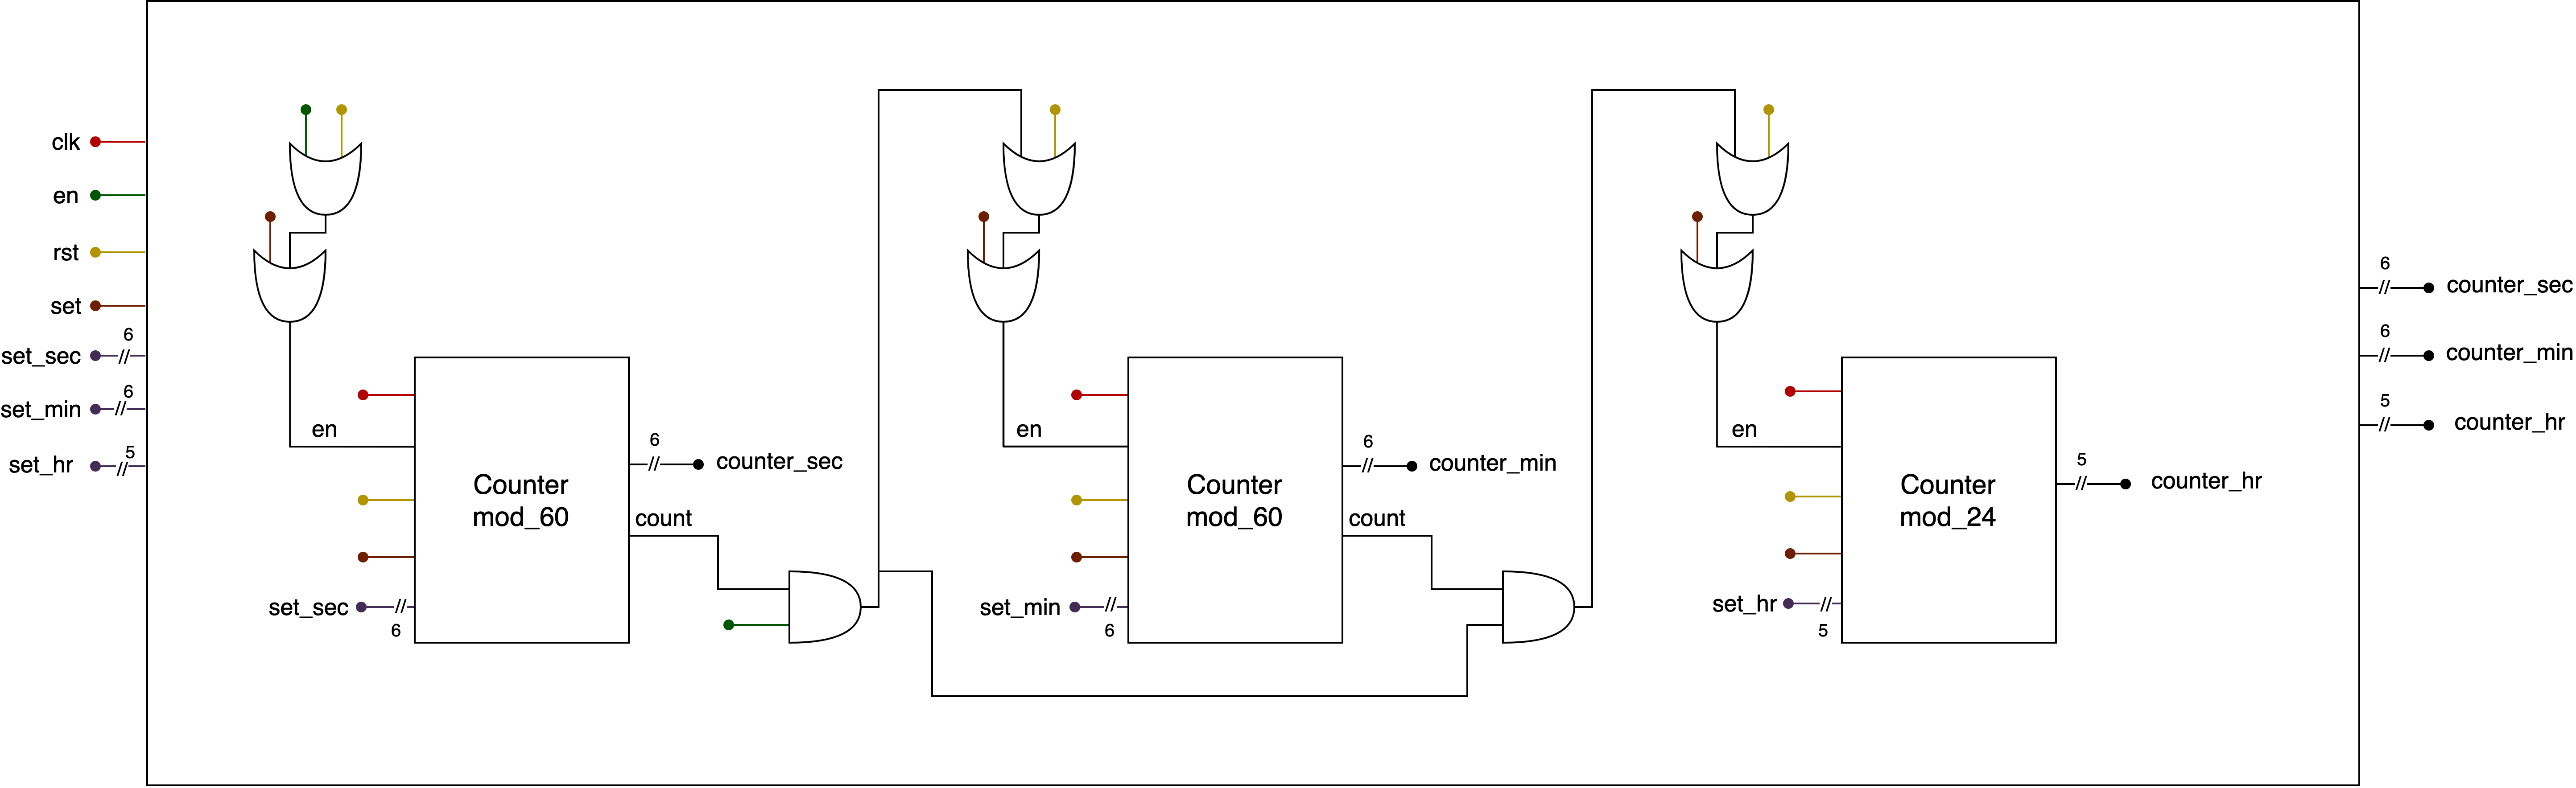
\includegraphics[width=1\textwidth]{img/stopwatch.png}
	\caption{Cronometro}
	\label{stpwth} 
\end{figure}

\subsection{Implementazione}
Si può a questo punto prcedere con l'implementazione in VHDL del nostro progetto, partendo dalle sue componenti.
\subsubsection{Flip-Flop D}
\begin{code}
    \inputminted[frame=lines, framesep=2mm, baselinestretch=1.2, bgcolor=LightGray, fontsize=\footnotesize, linenos]{vhdl}{vhdl_files/Esercizio_5.1/ffD.vhdl}
    \caption{ffD.vhdl}
    \label{lst:ffD}
\end{code}
Il Flip-Flop D è stato implementato con un approccio comportamentale e con reset sincrono.

\subsubsection{Contatore modulo 64}
Utilizzando il Flip-Flop D, si implementa ora il contatore mdoulo 64.
\begin{code}
    \inputminted[frame=lines, framesep=2mm, baselinestretch=1.2, bgcolor=LightGray, fontsize=\footnotesize, linenos]{vhdl}{vhdl_files/Esercizio_5.1/counter_mod_64.vhdl}
    \caption{counter\_mod\_64.vhdl}
    \label{lst:count_64}
\end{code}

\subsubsection{Contatore modulo 32}
In modo analogo, si procede per il contatore modulo 32.
\begin{code}
    \inputminted[frame=lines, framesep=2mm, baselinestretch=1.2, bgcolor=LightGray, fontsize=\footnotesize, linenos]{vhdl}{vhdl_files/Esercizio_5.1/counter_mod_32.vhdl}
    \caption{counter\_mod\_32.vhdl}
    \label{lst:count_32}
\end{code}

\subsubsection{Contatore modulo 60}
Si implemeta ora il contatore modulo 60, partendo da quello modulo 64.
\begin{code}
    \inputminted[frame=lines, framesep=2mm, baselinestretch=1.2, bgcolor=LightGray, fontsize=\footnotesize, linenos]{vhdl}{vhdl_files/Esercizio_5.1/counter_mod_60.vhdl}
    \caption{counter\_mod\_60.vhdl}
    \label{lst:count_60}
\end{code}

\subsubsection{Contatore modulo 24}
Analogamente al contatore modulo 60, si implementa il contatore modulo 24 a partire da quello di modulo 32.
\begin{code}
    \inputminted[frame=lines, framesep=2mm, baselinestretch=1.2, bgcolor=LightGray, fontsize=\footnotesize, linenos]{vhdl}{vhdl_files/Esercizio_5.1/counter_mod_24.vhdl}
    \caption{counter\_mod\_24.vhdl}
    \label{lst:count_24}
\end{code}

\subsubsection{Cronometro}
Si può finalmente implementare il cronometro, utilizzando gli ultimi due contatori implementati.
\begin{code}
    \inputminted[frame=lines, framesep=2mm, baselinestretch=1.2, bgcolor=LightGray, fontsize=\footnotesize, linenos]{vhdl}{vhdl_files/Esercizio_5.1/stopwatch.vhdl}
    \caption{stopwatch.vhdl}
    \label{lst:stopwatch}
\end{code}

\subsection{Simulazione}
Per la simulazione, si implementa il seguente testbench:
\begin{code}
    \inputminted[frame=lines, framesep=2mm, baselinestretch=1.2, bgcolor=LightGray, fontsize=\footnotesize, linenos]{vhdl}{vhdl_files/Esercizio_5.1/stopwatch_tb.vhdl}
    \caption{stopwatch\_tb.vhdl}
    \label{lst:stopwatch_tb}
\end{code}

Lanciando la simulazione si ha 
\begin{figure}[H]
	\centering
	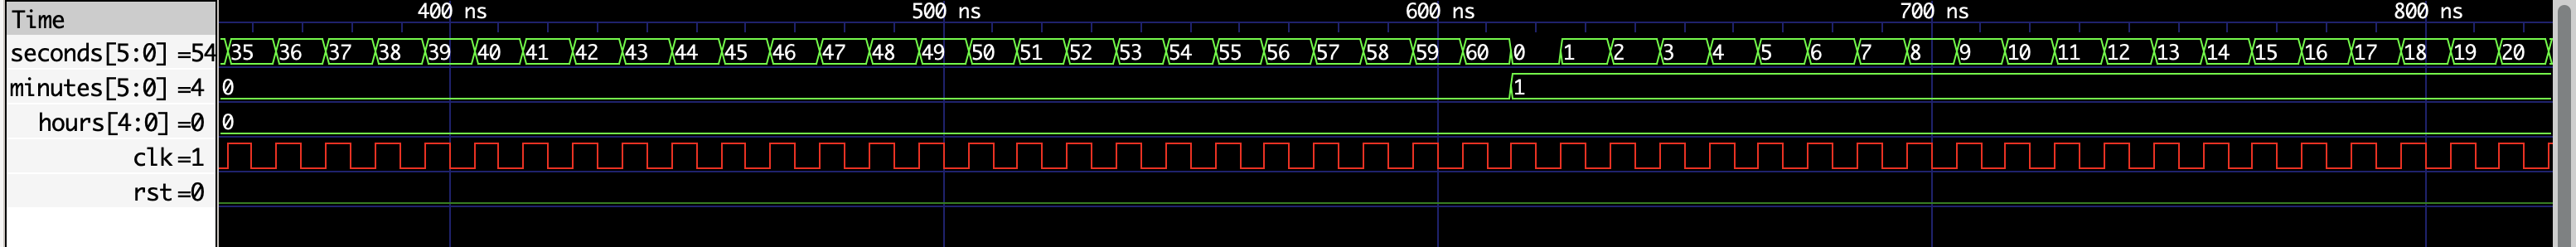
\includegraphics[width=1\textwidth]{img/stopwatch_sim}
	\caption{Simulazione Cronometro}
	\label{stpwth_sim} 
\end{figure}
Si vuole far notare che per materiali, è impossibile riportare nella documentazione l'intera simulazione.\\
Per cui qualore si volesse testare il cronometro, il codice VHDL si trova nella repository GitHub associata al progetto, nella cartella \texttt{Esercizio 5.1}.


%TODO: ADJUST THE STOPWATH ON BOARD 
\section{Implementazione su board del punto precedente}
\subsection{Traccia}
 Sintetizzare ed implementare su board il componente sviluppato al punto precedente, utilizzando i display a 7 segmenti per la visualizzazione dell’orario (o una combinazione di display e led nel caso in cui i display a disposizione siano in numero inferiore a quello necessario), gli switch per l’immissione dell’orario iniziale e due bottoni, uno per il set dell’orario e uno per il reset. Si utilizzi una codifica a scelta dello studente per la visualizzazione dell’orario sui display (esadecimale o decimale).
 \subsection{Implementazione}
 Per l'implementazione su board è stato necessario utilizzare il visore presente sulla board, per fare ciò sono stati usati i seguenti codici:
 \begin{code}
    \inputminted[frame=lines, framesep=2mm, baselinestretch=1.2, bgcolor=LightGray, fontsize=\footnotesize, linenos]{vhdl}{vhdl_files/cron_board/anodes_manager.vhd}
    \caption{anodes\_manager.vhdl}
    \label{lbl:ROMC}
\end{code}
 \begin{code}
    \inputminted[frame=lines, framesep=2mm, baselinestretch=1.2, bgcolor=LightGray, fontsize=\footnotesize, linenos]{vhdl}{vhdl_files/cron_board/anodes_manager.vhd}
    \caption{catode\_manager.vhdl}
    \label{lbl:ROMC}
\end{code}
 \begin{code}
    \inputminted[frame=lines, framesep=2mm, baselinestretch=1.2, bgcolor=LightGray, fontsize=\footnotesize, linenos]{vhdl}{vhdl_files/cron_board/display_seven_segments.vhd}
    \caption{display\_seven\_segments.vhdl}
    \label{lbl:ROMC}
\end{code}
\begin{code}
    \inputminted[frame=lines, framesep=2mm, baselinestretch=1.2, bgcolor=LightGray, fontsize=\footnotesize, linenos]{vhdl}{vhdl_files/cron_board/clock_filter.vhd}
    \caption{clock\_filter.vhdl}
    \label{lbl:ROMC}
\end{code}
\begin{code}
    \inputminted[frame=lines, framesep=2mm, baselinestretch=1.2, bgcolor=LightGray, fontsize=\footnotesize, linenos]{vhdl}{vhdl_files/cron_board/count_mod8.vhd}
    \caption{count\_mod8.vhdl}
    \label{lbl:ROMC}
\end{code}
Inoltre per avere una rappresentazione coerente sui visori, sono stati implementati i seguenti codici per distinguere decine e unità dalle uscite del cronometro:
 \begin{code}
    \inputminted[frame=lines, framesep=2mm, baselinestretch=1.2, bgcolor=LightGray, fontsize=\footnotesize, linenos]{vhdl}{vhdl_files/cron_board/separator.vhd}
    \caption{separator.vhdl}
    \label{lbl:ROMC}
\end{code}
 \begin{code}
    \inputminted[frame=lines, framesep=2mm, baselinestretch=1.2, bgcolor=LightGray, fontsize=\footnotesize, linenos]{vhdl}{vhdl_files/cron_board/sep_h_m_s.vhd}
    \caption{anodes\_manager.vhdl}
    \label{lbl:ROMC}
\end{code}
Si è inoltre scelto di usare un divisore di frequenza per ottenere un clock più adatto al funzionamento del progetto:
\begin{code}
    \inputminted[frame=lines, framesep=2mm, baselinestretch=1.2, bgcolor=LightGray, fontsize=\footnotesize, linenos]{vhdl}{vhdl_files/cron_board/freq_divider.vhd}
    \caption{freq\_divider.vhdl}
    \label{lbl:ROMC}
\end{code}
Per la gestione degli input, soprattutto relativi al \textit{SET} di secondi, minuti e ore, si è implementata una unotà di controllo, che sulla base del bottone premuto caricherà rispettivamente secondi (BTNU), minuti (BTNL) e ore (BTNR), e con un ulteriore bottone viene abilitato il SET (BTND). Inoltre con il bottone centrale si abilita il RESET.
\begin{code}
    \inputminted[frame=lines, framesep=2mm, baselinestretch=1.2, bgcolor=LightGray, fontsize=\footnotesize, linenos]{vhdl}{vhdl_files/cron_board/control_unit.vhd}
    \caption{control\_unit.vhdl}
    \label{lbl:ROMC}
\end{code}
La gestione del sistema nel suo complesso è implementata con il seguente codice:
\begin{code}
    \inputminted[frame=lines, framesep=2mm, baselinestretch=1.2, bgcolor=LightGray, fontsize=\footnotesize, linenos]{vhdl}{vhdl_files/cron_board/cron_onBOARD.vhd}
    \caption{cron\_onBoard.vhdl}
    \label{lbl:ROMC}
\end{code}
Si mostra anche il codice di Nexys-A7-50T-Master.xdc, fondamentale per la generazione del bitstream e di conseguenza per la programmazione della board.
{\footnotesize
\begin{verbatim}
## Clock signal
set_property -dict {PACKAGE_PIN E3 IOSTANDARD LVCMOS33}
[get_ports {CLK}]; #IO_L12P_T1_MRCC_35 Sch=clk100mhz
create_clock -add -name sys_clk_pin -period 10.00 -waveform {0 5} 
[get_ports {CLK}];

##Switches
set_property -dict {PACKAGE_PIN J15   IOSTANDARD LVCMOS33} 
[get_ports {value_in[0]}]; #IO_L24N_T3_RS0_15 Sch=sw[0]
set_property -dict { PACKAGE_PIN L16   IOSTANDARD LVCMOS33 } 
[get_ports { value_in[1] }]; #IO_L3N_T0_DQS_EMCCLK_14 Sch=sw[1]
set_property -dict { PACKAGE_PIN M13   IOSTANDARD LVCMOS33 } 
[get_ports { value_in[2] }]; #IO_L6N_T0_D08_VREF_14 Sch=sw[2]
set_property -dict { PACKAGE_PIN R15   IOSTANDARD LVCMOS33 } 
[get_ports { value_in[3] }]; #IO_L13N_T2_MRCC_14 Sch=sw[3]
set_property -dict { PACKAGE_PIN R17   IOSTANDARD LVCMOS33 } 
[get_ports { value_in[4] }]; #IO_L12N_T1_MRCC_14 Sch=sw[4]
set_property -dict { PACKAGE_PIN T18   IOSTANDARD LVCMOS33 } 
[get_ports { value_in[5] }]; #IO_L7N_T1_D10_14 Sch=sw[5]

##7 segment display
set_property -dict { PACKAGE_PIN T10   IOSTANDARD LVCMOS33 } 
[get_ports { cathodes_out[0] }]; #IO_L24N_T3_A00_D16_14 Sch=ca
set_property -dict { PACKAGE_PIN R10   IOSTANDARD LVCMOS33 } 
[get_ports { cathodes_out[1] }]; #IO_25_14 Sch=cb
set_property -dict { PACKAGE_PIN K16   IOSTANDARD LVCMOS33 } 
[get_ports { cathodes_out[2] }]; #IO_25_15 Sch=cc
set_property -dict { PACKAGE_PIN K13   IOSTANDARD LVCMOS33 } 
[get_ports { cathodes_out[3] }]; #IO_L17P_T2_A26_15 Sch=cd
set_property -dict { PACKAGE_PIN P15   IOSTANDARD LVCMOS33 } 
[get_ports { cathodes_out[4] }]; #IO_L13P_T2_MRCC_14 Sch=ce
set_property -dict { PACKAGE_PIN T11   IOSTANDARD LVCMOS33 } 
[get_ports { cathodes_out[5] }]; #IO_L19P_T3_A10_D26_14 Sch=cf
set_property -dict { PACKAGE_PIN L18   IOSTANDARD LVCMOS33 } 
[get_ports { cathodes_out[6] }]; #IO_L4P_T0_D04_14 Sch=cg
set_property -dict { PACKAGE_PIN H15   IOSTANDARD LVCMOS33 } 
[get_ports { cathodes_out[7] }]; #IO_L19N_T3_A21_VREF_15 Sch=dp
set_property -dict { PACKAGE_PIN J17   IOSTANDARD LVCMOS33 } 
[get_ports { anodes_out[0] }]; #IO_L23P_T3_FOE_B_15 Sch=an[0]
set_property -dict { PACKAGE_PIN J18   IOSTANDARD LVCMOS33 } 
[get_ports { anodes_out[1] }]; #IO_L23N_T3_FWE_B_15 Sch=an[1]
set_property -dict { PACKAGE_PIN T9    IOSTANDARD LVCMOS33 } 
[get_ports { anodes_out[2] }]; #IO_L24P_T3_A01_D17_14 Sch=an[2]
set_property -dict { PACKAGE_PIN J14   IOSTANDARD LVCMOS33 } 
[get_ports { anodes_out[3] }]; #IO_L19P_T3_A22_15 Sch=an[3]
set_property -dict { PACKAGE_PIN P14   IOSTANDARD LVCMOS33 } 
[get_ports { anodes_out[4] }]; #IO_L8N_T1_D12_14 Sch=an[4]
set_property -dict { PACKAGE_PIN T14   IOSTANDARD LVCMOS33 } 
[get_ports { anodes_out[5] }]; #IO_L14P_T2_SRCC_14 Sch=an[5]
set_property -dict { PACKAGE_PIN K2    IOSTANDARD LVCMOS33 } 
[get_ports { anodes_out[6] }]; #IO_L23P_T3_35 Sch=an[6]
set_property -dict { PACKAGE_PIN U13   IOSTANDARD LVCMOS33 } 
[get_ports { anodes_out[7] }]; #IO_L23N_T3_A02_D18_14 Sch=an[7]

##Buttons
#set_property -dict { PACKAGE_PIN C12   IOSTANDARD LVCMOS33 } 
[get_ports { reset_in }]; #IO_L3P_T0_DQS_AD1P_15 Sch=cpu_resetn
set_property -dict { PACKAGE_PIN N17   IOSTANDARD LVCMOS33 } 
[get_ports { RST }]; #IO_L9P_T1_DQS_14 Sch=btnc
set_property -dict { PACKAGE_PIN M18   IOSTANDARD LVCMOS33 } 
[get_ports { load_s }]; #IO_L4N_T0_D05_14 Sch=btnu
set_property -dict { PACKAGE_PIN P17   IOSTANDARD LVCMOS33 } 
[get_ports { load_m }]; #IO_L12P_T1_MRCC_14 Sch=btnl
set_property -dict { PACKAGE_PIN M17   IOSTANDARD LVCMOS33 } 
[get_ports { load_h }]; #IO_L10N_T1_D15_14 Sch=btnr
set_property -dict { PACKAGE_PIN P18   IOSTANDARD LVCMOS33 } 
[get_ports { SET }]; #IO_L9N_T1_DQS_D13_14 Sch=btnd


\end{verbatim}
}


\chapter{Esercizio 6}
\section{Sistema di lettura - elaborazione - scrittura PO\_PC}
\subsection{Traccia}
 Progettare, implementare in VHDL e verificare mediante simulazione un sistema dotato di una memoria ROM di N locazioni da 8 bit ciascuna, una macchina combinatoria M in grado di trasformare (secondo una funzione a scelta dello studente) la stringa di 8 bit letta dalla ROM in una stringa di 4 bit, e una memoria MEM di N locazioni che memorizza la stringa in output da M. Il sistema si avvia in corrispondenza di un segnale di START che viene fornito esternamente. Una volta avviato, tramite un’apposita unità di controllo che gestisce la tempificazione del sistema, viene scandita una locazione alla volta della ROM e viene scritta la corrispondente locazione di MEM. Gli indirizzi di memoria sono forniti da un contatore. Le memorie ROM e MEM hanno rispettivamente un read e un write sincrono.
\subsection{Progettazione}
Per il progetto di questo sistema si riprende l'esercizio nel capitolo 2: \textbf{Sistema ROM + M}. Viene usato anche un contatore, per scandire una alla volta tutte le locazioni della ROM da cui prelevare la stringa contenente 8 bit. Come nell'esercizio precedente, l'uscita della ROM viene posta in ingresso alla macchina M, che somma i 4 bit più significativi dell'ingresso con i 4 bit meno significativi. L'uscita della macchina M viene posto in ingresso a una memoria MEM e poi caricato nella locazione corrispondente all'uscita del contatore; il funzionamento del sistema viene gestito da un'unità di controllo.  
La struttura del sistema sarà fatta in questo modo:
\begin{figure}[H]
	\centering
	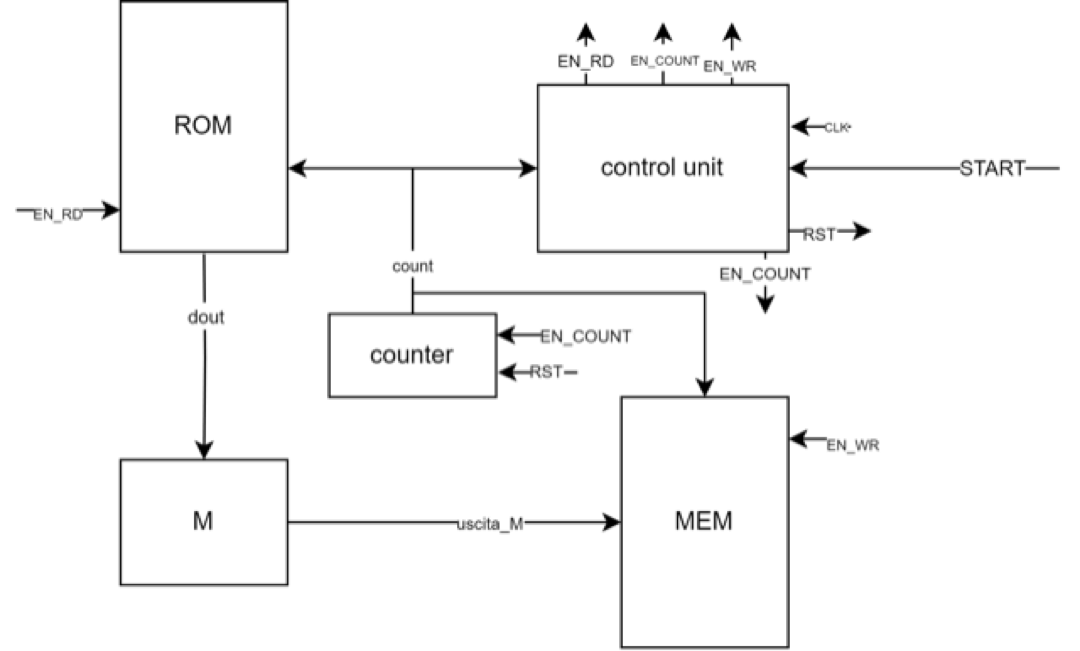
\includegraphics[width=1\textwidth]{img/ROM_M_MEM.png}
	\caption{Schema a blocchi del sistema ROM + M + MEM}
	\label{shf_reg_beh_sim} 
\end{figure}
L'unità di controllo (CU) può essere efficacemente modellata come una macchina a stati finiti (FSM). Nel caso particolare avremo i seguenti stati:
\begin{itemize}
    \item \textbf{idle}
    \item \textbf{read}
    \item \textbf{m\_work}
    \item \textbf{write}
\end{itemize}
L'unità di controllo può essere quindi rappresentata da un automa come si mostra in figura:
\begin{figure}[H]
	\centering
	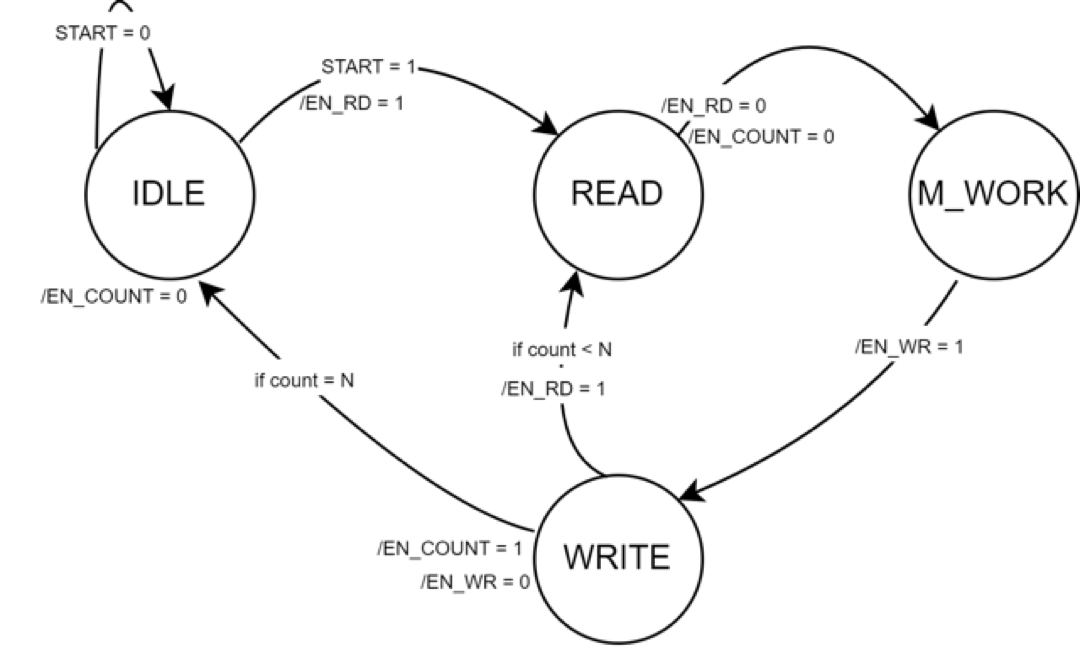
\includegraphics[width=1\textwidth]{img/Automa_ROM_M_MEM.png}
	\caption{Macchina a stati della control unit di ROM + M + MEM}
	\label{automa_rom_m_mem} 
\end{figure}
\subsection{Implementazione}
Il codice implementativo di M resta invariato, in quanto macchina puramente combinatoria. Si nota che viene richiesto che le operazioni di Read dalla ROM e di Write sulla memoria MEM siano svolte in modo sincrono. Quindi, a differenza della ROM usata nell'esercizio precedente, che era puramente combinatoria, le operazioni di lettura di questa ROM avvengono in sincronia con un segnale di clock. Questo segnale fornisce un riferimento temporale preciso per tutte le operazioni interne della ROM, garantendo così un funzionamento coerente e affidabile. Inoltre, sono stati utilizzati dei segnali di abilitazione alla lettura e alla scrittura, in modo da evitare conflitti e da permettere che i dati vengano letti al momento giusto. 
Si mostra innanzitutto il nuovo codice di ROM:
\begin{code}
    \inputminted[frame=lines, framesep=2mm, baselinestretch=1.2, bgcolor=LightGray, fontsize=\footnotesize, linenos]{vhdl}{vhdl_files/ROM_MEM_M/ROMconCLOCK.vhd}
    \caption{ROM.vhdl}
    \label{lbl:ROMC}
\end{code}
Si è scelto di utilizzare le stesse stringhe dell'esercizio 2 per "popolare" la ROM, in modo da poter confrontare i risultati.
Si mostra ora l'implementazione dell'unità di controllo del sistema; tale codice gestisce i cambiamenti di stato, e si può considerare il "cervello" del sistema in esame. \\
Si noti che si è scelto di porre in uscita gli stati, in modo da visualizzare in simulazione anche le variazioni di stato, è una scelta ovviamente facoltativa, ma per ragione di debugging è stato scelto di visualizzare anche la variazione di stato, come sarà visibile dalla waveform nella prossima sezione.
\begin{code}
    \inputminted[frame=lines, framesep=2mm, baselinestretch=1.2, bgcolor=LightGray, fontsize=\footnotesize, linenos]{vhdl}{vhdl_files/ROM_MEM_M/control_unit.vhd}
    \caption{control unit.vhdl}
    \label{lbl:ROMC}
\end{code}
Si mostra infine il codice sistema nel suo complesso, composto dall'unità di controllo e da tutte le altre componenti utilizzate; è stato utilizzato un approccio di tipo strutturale:
\begin{code}
    \inputminted[frame=lines, framesep=2mm, baselinestretch=1.2, bgcolor=LightGray, fontsize=\footnotesize, linenos]{vhdl}{vhdl_files/ROM_MEM_M/ROM_M_MEMO.vhd}
    \caption{ROM + M + MEM.vhdl}
    \label{lbl:ROMC}
\end{code}
Si vuole porre l'attenzione allo Schematic generato dall'ambiente Vivado, che mostra chiaramente i collegamenti e le dipendenze tra tutte le componenti del sistema.
\begin{figure}[H]
	\centering
	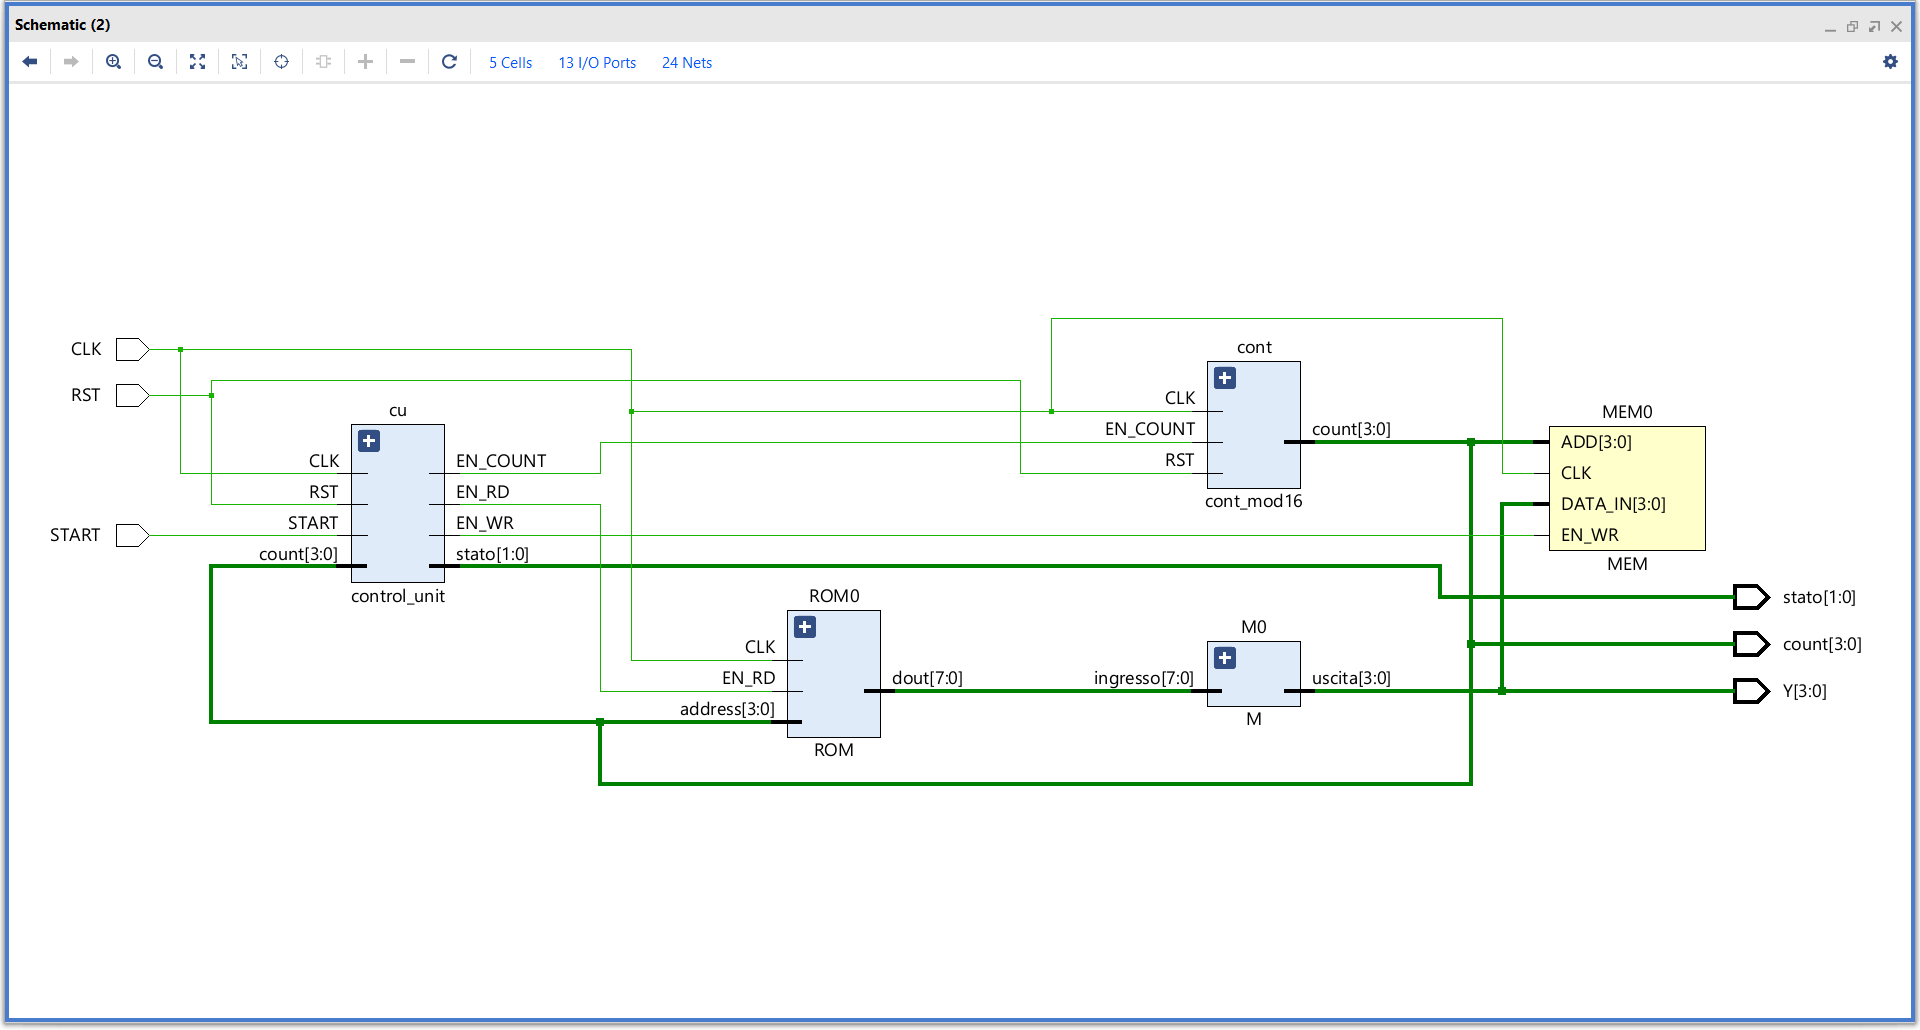
\includegraphics[width=1\textwidth]{img/schematic_ROM_M_MEM.PNG}
	\caption{Schematic di ROM + M + MEM}
	\label{schemROM_M_MEM} 
\end{figure}
\subsection{Simulazione}
Per procedere con la simulazione è stato necessario generare un testbench:
\begin{code}
    \inputminted[frame=lines, framesep=2mm, baselinestretch=1.2, bgcolor=LightGray, fontsize=\footnotesize, linenos]{vhdl}{vhdl_files/ROM_MEM_M/Rom_M_MEM_tb.vhd}
    \caption{Testbench di ROM + M + MEM.vhdl}
    \label{lbl:ROMC}
\end{code}
Eseguendo la simulazione si avrà la seguente forma d'onda:
\begin{figure}[H]
	\centering
	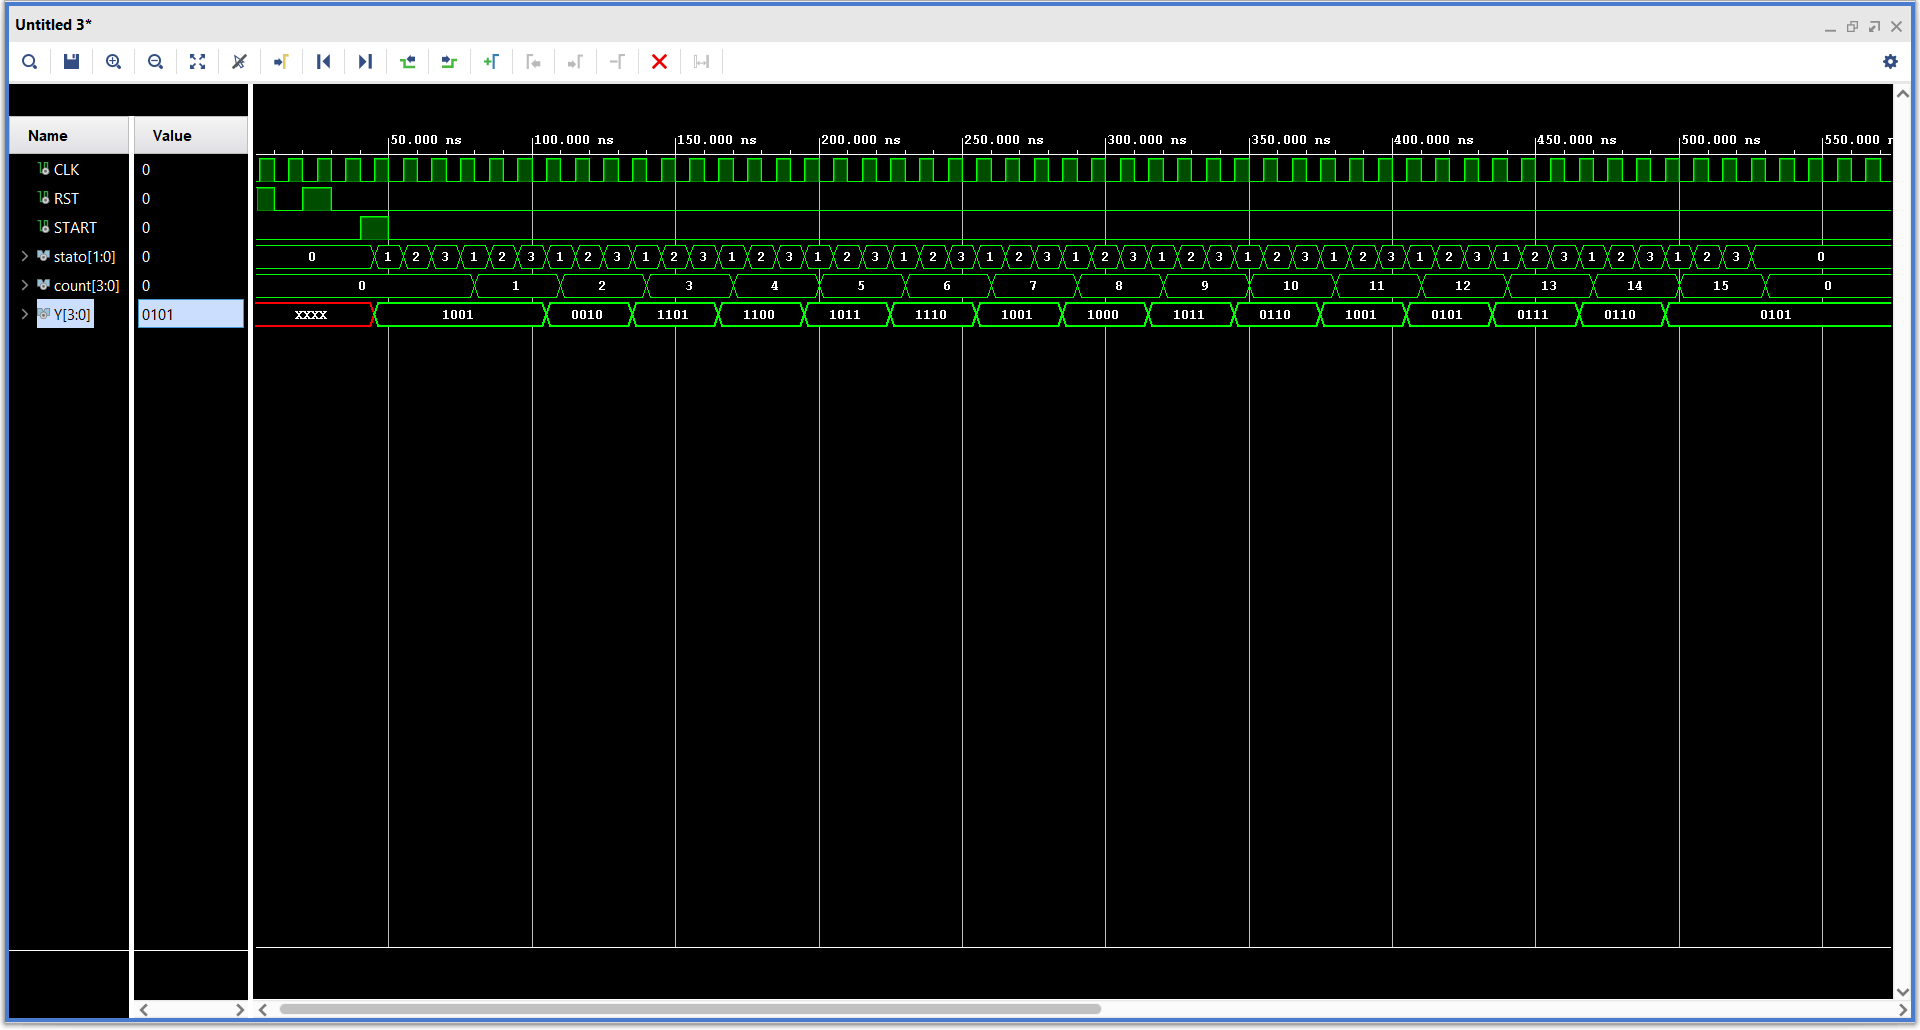
\includegraphics[width=1\textwidth]{img/ROM_M_MEM_waweform.PNG}
	\caption{Waveform di ROM + M + MEM}
	\label{schemROM_M_MEM} 
\end{figure}
Si analizzano alcuni casi per dimostrare la correttezza del sistema.
\begin{itemize}
    \item \textbf{istante 0:} si accede alla locazione di memoria $0$, in cui si trova la stringa $"00001001"$, sommando i 4 bit più significativi con i 4 meno significativi si ottiene $1001$;
    \item \textbf{istante 1:} si accede alla locazione di memoria $1$, in cui si trova la stringa $"10001010"$, all'uscita della macchina M si ottiene $0010$;
   \item \textbf{istante 2:} si accede alla locazione di memoria $2$, in cui si trova la stringa $"00001101"$, procedendo come in precedenza si ottiene $1101$.
\end{itemize}
Si può procedere in questo modo per tutte le locazioni di memoria scandite dal contatore confermando così il risultato della simulazione.\\
Come detto, si è scelto di mostrare anche le variazioni dello stato e del contatore, in modo da avere la possibilità di osservare in ogni istante il comportamento del sistema, tale scelta è del tutto opzionale.
\section{Implementazione su board del punto precedente}
\subsection{Traccia}
Sintetizzare ed implementare su board il componente sviluppato al punto 
precedente, utilizzando due bottoni per i segnali di read e reset rispettivamente e i 
led per la visualizzazione delle uscite della macchina istante per istante.
\subsection{Implementazione}
Nel caso in esame, per procedere all'implementazione su board, è stato necessario apportare alcune modifiche: viene infatti richiesto che la lettura sia abilitata da un segnale esterno proveniente da un bottone della board, mentre nell'implementazione precedente, l'abilitazione alla lettura era un'uscita dell'unità di controllo, che veniva posta alta o bassa in base allo stato corrente. in ogni caso, i codici di ROM, M, counter e MEM restano invariati rispetto al punto precedente, e vengono quindi semplicemente importati.\\
Si dimostra inoltre necessario l'utilizzo di un divisore di frequenza, componente che si importa dagli esercizi precedenti, per cui non si riporta nuovamente il codice.\\
Si procede quindi a mostrare le modifiche apportate all'implementazione dell'unità di controllo e di $ROM\_M\_M.vhdl$ per la gestione dell'$EN\_RD$ come segnale di ingresso dalla board.
\begin{code}
    \inputminted[frame=lines, framesep=2mm, baselinestretch=1.2, bgcolor=LightGray, fontsize=\footnotesize, linenos]{vhdl}{vhdl_files/ROM_M_MEM_board/control_unit.vhd}
    \caption{Control Unit con EN\_RD come ingresso}
    \label{lbl:ROMC}
\end{code}
\begin{code}
    \inputminted[frame=lines, framesep=2mm, baselinestretch=1.2, bgcolor=LightGray, fontsize=\footnotesize, linenos]{vhdl}{vhdl_files/ROM_M_MEM_board/Rom_M_MEM.vhd}
    \caption{ROM + M + MEM su board}
    \label{lbl:ROMC}
\end{code}
Si nota che le uscite commentate nel codice (stato e count) sono state utilizzate ai fini del debugging, per monitorare che le uscite corrispondessero alla giusta locazione di memoria e che i cambiamenti di stato avvenissero in maniera efficiente.\\
Si è scelto inoltre di mostrare attraverso $led 15$ della board anche le variazioni del clock, per un'ulteriore conferma visiva della correttezza del sistema.\\
Come si deduce dal codice mostrato, è stato scelto di usare 3 bottoni per gestire il funzionamento del sistema, $BTNU$ come ingresso per $START$, $BTNL$ come ingresso per $EN\_RD$ e $BNTC$ come ingresso per $reset$; per consentire ciò i collegamenti sono stati aggiunti nel file $Nexys-A7-50T-Master.xdc$.\\
Si mostrano ora i riultati ottenuti sulla board, avendo dato l'abilitazione alla lettura in 3 istanti diversi.
\begin{figure}[H]
	\centering
	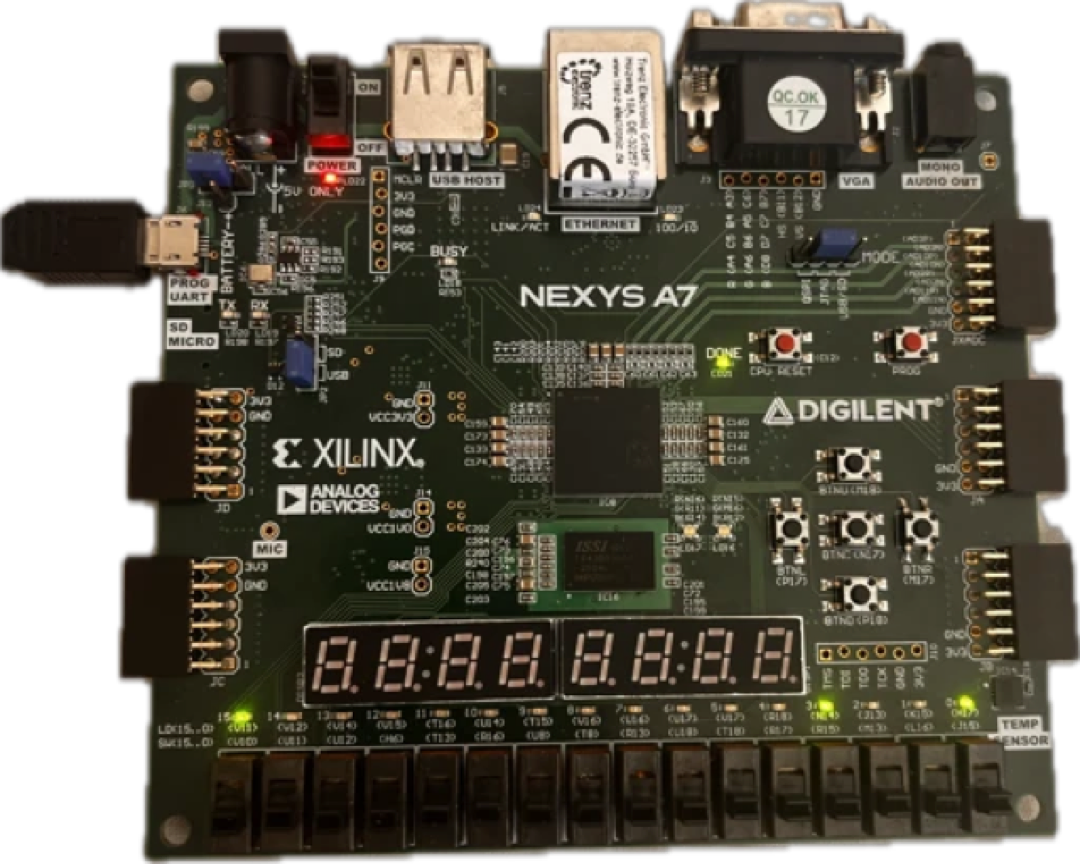
\includegraphics[width=0.7\textwidth]{img/Test1_ROM_M_MEMwebp.png}
	\caption{Istante 0: uscita = $1001$}
	\label{schemROM_M_MEM} 
\end{figure}

\begin{figure}[H]
	\centering
	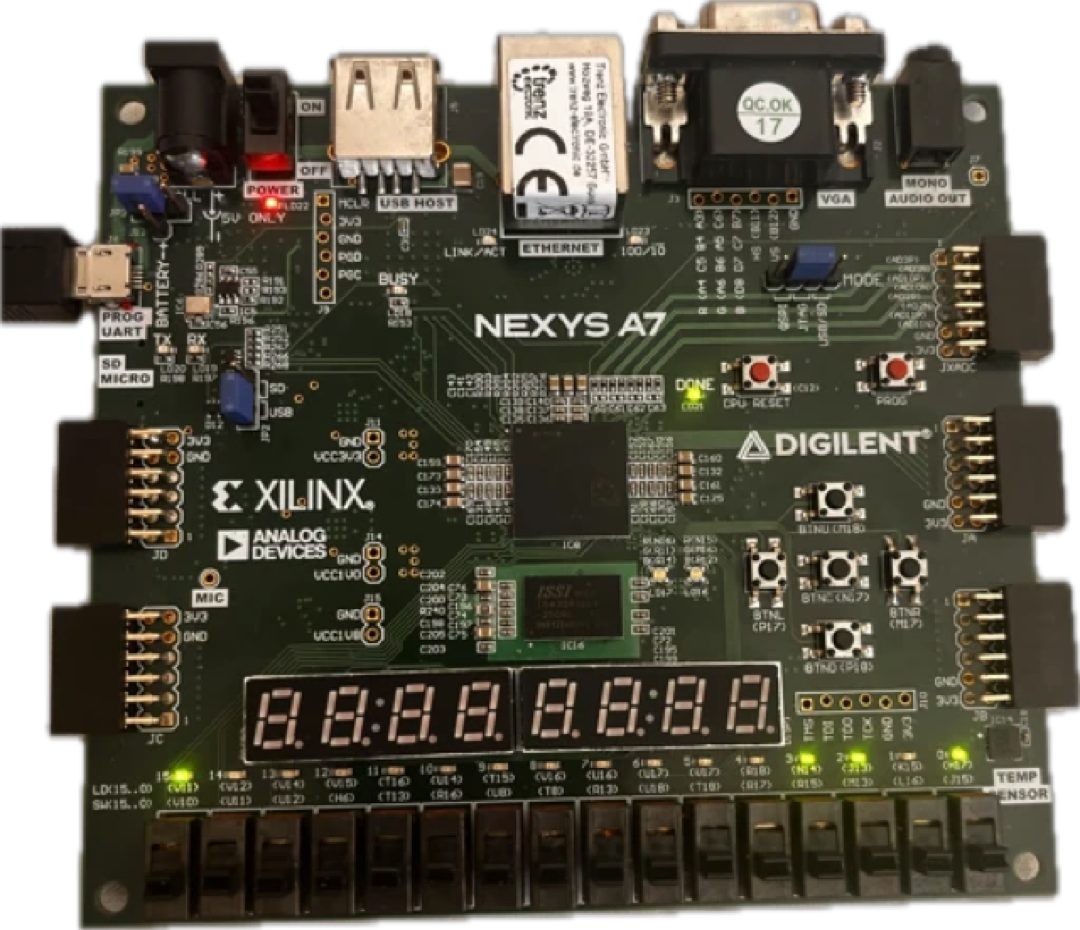
\includegraphics[width=0.7\textwidth]{img/Test2_ROM_M_MEMwebp.png}
	\caption{Istante 2: uscita = $1101$}
	\label{schemROM_M_MEM} 
\end{figure}


\begin{figure}[H]
	\centering
	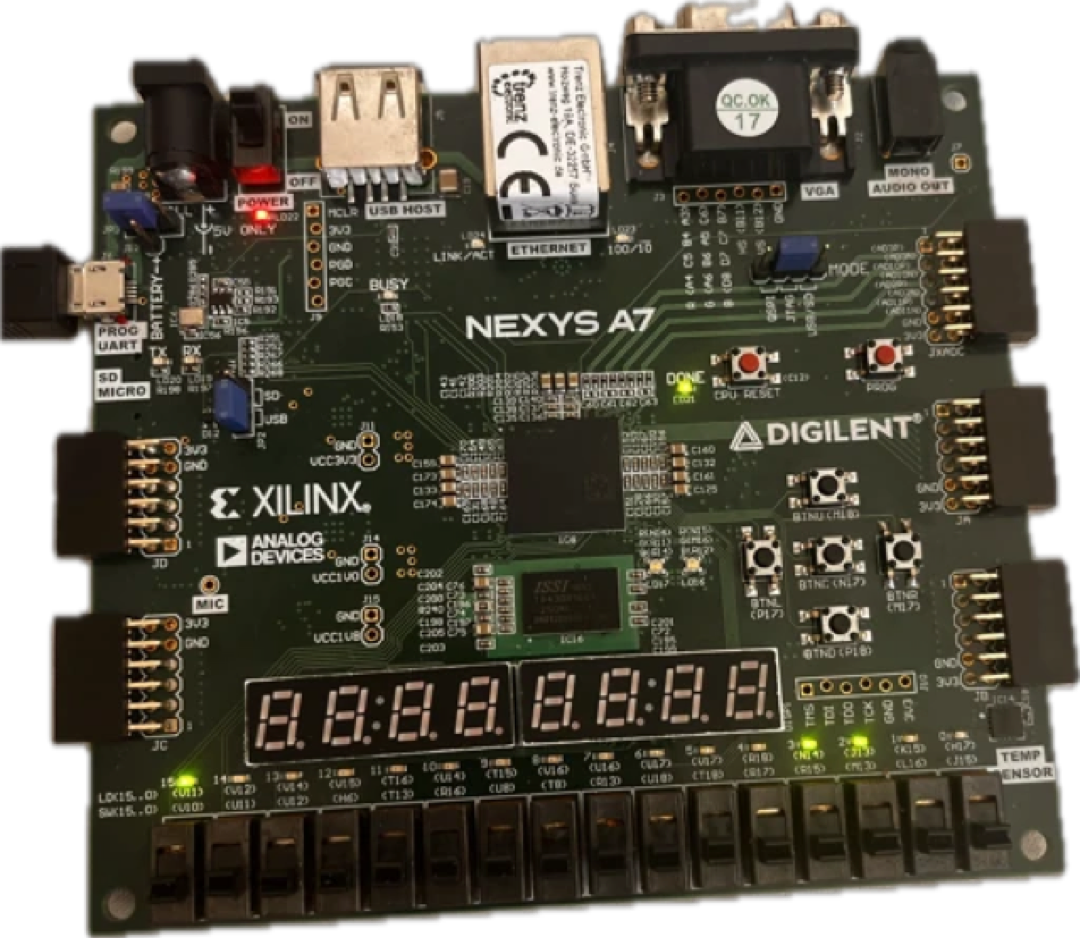
\includegraphics[width=0.7\textwidth]{img/Test3_ROM_M_MEMwebp.png}
	\caption{Istante 3: uscita = $1100$}
	\label{schemROM_M_MEM} 
\end{figure}
